\documentclass[12pt]{article}
\usepackage{amssymb,amsmath,natbib,graphicx,amsthm,
  setspace,sectsty,anysize,times,dsfont,enumerate}

\usepackage[svgnames]{xcolor}

\usepackage{lscape,arydshln,relsize,rotating,multirow}
\usepackage{caption}
\captionsetup{%
  font=small,
  labelfont=normalfont,
  singlelinecheck=false,
  justification=justified
}
\usepackage{algorithm}

\graphicspath{{/Users/mtaddy/project/gamma_lasso/graphs/}}
\newtheorem{prop}{\sc Proposition}[section]
\newtheorem{theorem}{\sc Theorem}[section]
\newtheorem{definition}{\sc Definition}[section]
\newtheorem{lemma}{\sc Lemma}[section]
\newtheorem{corollary}{\sc Corollary}[section]

\marginsize{1.1in}{.9in}{.3in}{1.4in}

\newcommand{\nb}{\color{blue}}
\newcommand{\dbl}{\setstretch{1.5}}
\newcommand{\sgl}{\setstretch{1.1}}

\newcommand{\bs}[1]{\boldsymbol{#1}}
\newcommand{\mc}[1]{\mathcal{#1}}
\newcommand{\mr}[1]{\mathrm{#1}}
\newcommand{\bm}[1]{\mathbf{#1}}
\newcommand{\ds}[1]{\mathds{#1}}
\newcommand{\indep}{\perp\!\!\!\perp}
\DeclareMathOperator*{\argmin}{argmin}
\newcommand{\norm}[1]{|\!|#1|\!|_{1}}
\newcommand{\code}[1]{{\smaller\sf#1}}
\newcommand{\e}[1]{{\footnotesize$\times10$}{$^{#1}$}}

\sectionfont{\noindent\normalfont\large\bf}
\subsectionfont{\noindent\normalfont\normalsize\bf}
\subsubsectionfont{\noindent\normalfont\it}

\usepackage[bottom,hang,flushmargin]{footmisc}

\pdfminorversion=4
\begin{document}

\sgl 

\pagestyle{empty}

~
\vskip 3cm

\noindent {\huge \bf The Gamma Lasso} 

\vskip 1cm

\noindent{\Large Matt Taddy}

{\large
\vskip .5cm \noindent
{The  University of Chicago Booth School of Business}\\
{\tt faculty.chicagobooth.edu/matt.taddy}}



\vskip 2cm

{\noindent This article describes a very fast algorithm for obtaining
continuous regularization paths corresponding to cost functions spanning the
range of concavity between $L_0$ and $L_1$ norms.  The `gamma lasso' heuristic
does $L_1$ (lasso) penalized regression estimation on a grid of decreasing
penalties, but adapts coefficient-specific weights to decrease as a function
of the estimated coefficient in the previous path segment.  This  simple
recipe is used to review the literature on diminishing bias penalty regularization,
emphasizing connections to weighted $L_1$ penalties, the role of regularization paths and model selection, and the distance from a weighted lasso
solution to an $L_0$ penalized oracle. The work is illustrated in
extensive linear regression simulations and in application of logistic
regression to evaluate the performance of hockey players.}
 

\newpage
\dbl

\pagestyle{plain}
\vskip 1cm
\section{Introduction}
\label{intro}

For regression in high-dimensions it is useful to regularize estimation
through a penalty on coefficient size.   This article introduces a very fast
algorithm, the {\it gamma lasso}, for $L_1$ penalty regularization with a
data-dependent weight on the cost of each coefficient. The algorithm  serves
as a basis for exploring the world of sparse {\it diminishing bias}
regularization, where penalties are spiked at zero  but have costs diminish so as to remove bias from estimation of large
signals.

We introduce regularization path estimation in Section \ref{intro}.1, before
detailing the gamma lasso (GL) algorithm in  \ref{intro}.2. Briefly, GL solves
a path of weighted $L_1$ penalized estimators with  weights at each segment a
function of coefficient estimates at the previous segment.  Section
\ref{bayes} derives a Bayesian foundation, while Section \ref{concave}
connects concave and  weighted $L_1$ penalization.

% The gamma lasso is not a radically new idea.  Indeed, this
% article is intended to provide a review, wrapping up the material necessary for practical
% application of diminishing bias estimators.  Big Data application of such tools
% nearly always leads to a version of weighted $L_1$ regularization.  Our new
% approach learns from the literature to provide a much more practically
% effective and scalable algorithm than currently exists. However, we are not
% claiming {\it theoretical} optimality of the gamma lasso, and if others wish
% to claim superiority for their methods this article should help build
% perspective on what should be considered during implementation.


One theme of our work holds that sparse estimation will be useful for (and
often used in) settings where the true data generating process is non-sparse.
This can be motivated from an information compression  perspective -- e.g., in
Big data settings such as
\cite{taddy_distributed_2013}, where many estimates need to be quickly
communicated across multiple machines -- or from a simple desire to minimize
complexity and focus decision making.   In these cases, diminishing bias 
helps get fits that are {\it as sparse as possible} while still being useful
for prediction. Section \ref{theory} presents theoretical results on the
distance between weighted $L_1$ estimation and an $L_0$ penalized oracle
(rather than  some assumed sparse truth), and Section
\ref{sim} provides a simulation study.

Another central view of this work is that GL and related
techniques from sparse regularization do not actually {\it do} model
selection; rather, the paths of estimators corresponding to different levels
of penalization provide a set of candidates from which one must choose. It is
essential that these paths are evaluated as a whole, and that they are good platforms for model selection. Section
\ref{stability} studies path stability, focusing on implications for
algorithm speed and for predictor
variance.  Section \ref{dof} describes a heuristic for model
degrees of freedom, and Section \ref{selection} details cross validation and
information criteria as tools for model selection.

Finally,  Section \ref{nhl} explores all of these ideas in a high-dimensional inference problem: given all goals in the past decade of NHL hockey, and information about who was on the ice, what can we say about individual player contributions?  We'll explore how various degrees of diminishing bias lead to different conclusions, ranging from a world where rookies are among the best in the league and another where only established stars have any measurable effect.


\subsection{Regularization paths}

Denote $n$ response observations as $\bm{y} = [y_1,\ldots,y_n]'$ and the associated matrix of $p$ covariates as $\bm{X} =
[\bm{x}_1 \cdots \bm{x}_n]'$, with rows $\bm{x}_i = [x_{i1},\ldots,x_{ip}]'$ and columns $\bs{x}_j = [x_{1j},\ldots,x_{nj}]'$.\footnote{Since the size of penalized $\beta_j$ depends upon the units of $x_{ij}$,  it is common to scale
the coefficient by $\mr{sd}(\bs{x}_j)$, the standard deviation of the $j^{th}$ column
of $\bm{X}$; this is achieved if $x_{ij}$ is replaced by $x_{ij}/\mr{sd}(\bs{x}_j)$
throughout.} Write $\eta_{i} =
\alpha+\bm{x}_i'\bs{\beta}$ as the linear equation for observation $i$, and
denote with $l(\alpha, \bs{\beta}) = l(\bs{\eta})$  an unregularized
objective  proportional to the negative log likelihood.  For example, in Gaussian (linear)
regression, $l(\bs{\eta})$ is the sum-of-
squares $0.5\sum_i \left(y_i - \eta_i\right)^2$ and in binomial (logistic)
regression,  $l(\bs{\eta}) = -\sum_i \left[\eta_iy_i -
\log(1+e^{\eta_i})\right]$ for $y_i \in [0,1]$.  
A penalized estimator is then the solution to
\begin{equation} \label{pendev}
{\min}\left\{~l(\alpha,{\bs{\beta}}) + n\lambda \sum_{j=1}^p c_j(|\beta_j|)~\right\},
\end{equation}
where $\lambda>0$ controls overall penalty magnitude and are $c_j()$ are coefficient cost functions.

\begin{figure}[t]
\vspace{-.5cm}
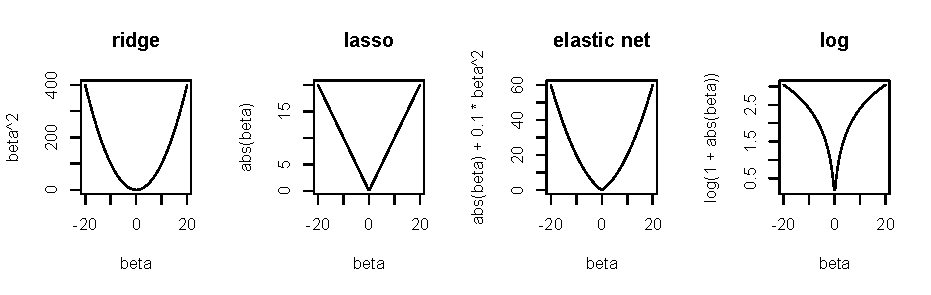
\includegraphics[width=6.25in]{penalties}
\vskip -.5cm
\caption{\label{costs} 
From left to right, 
$L_2$ costs \citep[ridge,][]{hoerl_ridge_1970}, $L_1$ \citep[lasso,][]{tibshirani_regression_1996}, the `elastic net' mixture of $L_1$ and $L_2$ \citep{zou_regularization_2005}, and the log penalty \citep{candes_enhancing_2008}.
}
\end{figure}

A few common cost functions are shown in Figure \ref{costs}.  Those that have
a non-differentiable spike at zero (all but ridge) lead to sparse estimators,
with some coefficients set to exactly zero.   The curvature of the penalty
away from zero dictates then the weight of shrinkage imposed on the nonzero
coefficients:  $L_2$ costs increase with coefficient size,  lasso's $L_1$
penalty has zero curvature and imposes constant shrinkage, and as curvature
goes towards $-\infty$ one approaches the $L_0$ penalty of subset selection.
In this article we are primarily interested in {\it concave} cost functions,
like the log penalty, which span the range between $L_1$ and $L_0$ penalties.

The penalty size, $\lambda$, acts as a {\it squelch}: it suppresses noise to
focus on the true input signal. Large $\lambda$ lead to very simple 
model estimates, while as $\lambda \rightarrow 0$ we approach maximum
likelihood estimation (MLE). Since you don't know optimal $\lambda$,
practical application of penalized estimation requires a {\it regularization
path}: a $p \times T$ field of $\bs{\hat\beta}$ estimates obtained while
moving from high to low penalization along $\lambda^1 > \lambda^2 \ldots >
\lambda^T$ \citep[e.g., LARS in][is a well known example]{efron_least_2004}.
These paths begin at $\lambda^1$ set to infimum $\lambda$ such that
(\ref{pendev}) is minimized at $\bs{\hat\beta} = \bm{0}$ (see Appendix
\ref{models}), and proceed down to some pre-specified $\lambda^T$ (e.g., $\lambda^T=
0.01\lambda^1$).

Given a regularization path, the selection problem is to choose $\lambda$
so that models estimated under that  squelch are neither over nor under fit.
For this reason, it is essential that the paths provide good material for
model selection.  In Section \ref{stability} and afterwards, we see that path
{\it stability} is a key property.  This is closely linked with the
rate of change in $\bs{\hat\beta}$ as a function of $\lambda$.  At the very
least, one desires coefficient paths  smooth enough that $\bs{\hat\beta}^t$ at
$\lambda^t$ provide {\it hot-starts} for $\bs{\hat\beta}^{t+1}$ at the next
penalty level. In this case, obtaining an entire regularization path
is  computationally efficient -- often requiring less time than for fit under
a single $\lambda$ from cold-start initialization.


\begin{figure}[thb]
\hskip -.2cm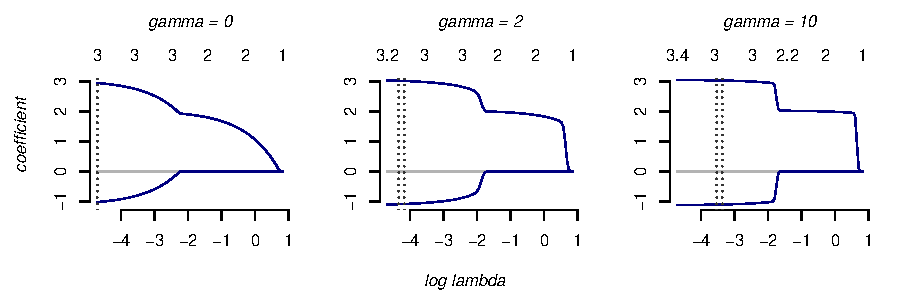
\includegraphics[width=6.5in]{gamlr_eg}
\vskip -.25cm
\caption{\label{gamlr_eg} Gamma lasso estimation on $n=10^3$ 
 observations of $y_i = 4 + 3x_{1i} - x_{2i} + \varepsilon_i$, where
$\varepsilon_i \stackrel{ind}{\sim} \mr{N}(0,1)$ and
$\{x_{1i},x_{2i},x_{3i}\}$ are marginally standard normal with correlation of
0.9 between covariates ($x_{3i}$ is spurious). The penalty path has $T=100$
segments, $\lambda^1 = n^{-1}\left| \sum_i x_{1i}y_i\right|$, and
$\lambda^{100} = 0.01\lambda^1$. Degrees of freedom are on top and vertical
lines mark AICc and BIC selected models (see Sections
\ref{dof}-\ref{selection}).}
\vskip -.25cm
\end{figure}


\subsection{The gamma lasso}
\label{glsec}

Diminishing bias is achieved if $L_1$ costs $c_j(\beta_j) = \omega_j
|\beta_j|$ use weights that  shrink for large $|\beta_j|$. The gamma lasso in
Algorithm \ref{gammalasso}, for `scale' $\gamma \geq 0$, yields paths of
penalized coefficient estimates $\bs{\hat\beta}^1 \ldots
\bs{\hat\beta}^T$ (and intercepts $\hat\alpha^1 \ldots \hat\alpha^T$)
corresponding to $L_1$ penalties $\lambda^1 > \lambda^2 \ldots > \lambda^T$
multiplied against adaptive coefficient-specific weight adjustments
$\bs{\omega}^1 \ldots \bs{\omega}^T$.

{\sgl\vskip.5cm
\begin{algorithm}[ht]
\caption{\label{gammalasso} The gamma lasso }
\vskip .2cm
Initialize $\bs{\omega}^1 = \bf{1}$ and $\lambda^1 >
0$ with step size
$0 < \delta < 1$.

\vspace{-.75cm}
\begin{align}
\text{for}~t=1\ldots T :&\notag \\
\left[\hat\alpha,\bs{\hat\beta}\right]^t &= \argmin_{\alpha,\beta_j\in\ds{R}}~~
l(\alpha,\bs{\beta}) + n\sum_j \lambda^t\omega^t_j|\beta_j| \label{l1pen}\\
\omega^{t+1}_j  &= \left(1 + \gamma |\hat\beta^t_j|\right)^{-1} ~~j=1\ldots p \label{adjweight}\\
\lambda^{t+1} &= \delta \lambda^t\notag
\end{align}
\vskip -.3cm
\end{algorithm}}

\noindent
Behavior of the GL paths  is governed by $\gamma$, which we refer to as the
penalty scale (see Section
\ref{bayes}).  Under $\gamma=0$ Algorithm \ref{gammalasso} is just the usual lasso.
 Bias diminishes faster for larger $\gamma$ and, at the  extreme,
$\gamma=\infty$ yields a subset selection routine where a coefficient is
unpenalized in all segments after it first becomes nonzero. Figure
\ref{gamlr_eg} shows solutions in a simple problem.

% Consider two steps of a single-covariate least-squares GL path, moving from penalty size $\lambda$ to $\delta\lambda$ for $0<\delta<1$.  Given MLE $b$ we can write
% the second segment estimator (at $\delta\lambda$) as \begin{equation}\label{twostep} f(b) = \left(b -
% \frac{\delta\lambda}{1+\gamma(b-\lambda)_+}\right)_+  \end{equation} where
% $\gamma,\lambda,\delta >0$, $\lambda < \infty$, $\delta<1$.  We call this the
% gamma-lasso thresholding operator, and it is straightforward to verify
% directly that it is Lipschitz continuous for $\gamma < \infty$.\footnote{}
% }  


\subsection{Implementation}

Each  gamma lasso path segment is solved through coordinate descent,
as detailed in Appendix \ref{implement}.  The algorithm is implemented in {\tt
c} as part of the {\tt gamlr} package for {\sf R}. This software is available
with documentation on {\tt cran.r-project.org} and versioned source code is at
{\tt github.com/mataddy/gamlr}.  Usage of {\tt gamlr} mirrors that of its
convex penalty analogue {\tt glmnet} \citep{friedman_regularization_2010}, the
fantastic and widely used package for costs between $L_1$ and $L_2$ norms. In
the lasso case ($\gamma=0$), the two algorithms are essentially equivalent.


\section{Bayesian motivation}
\label{bayes}

Consider a model where each $\beta_j$ is
assigned a Laplace distribution prior with scale $\tau_j>0$,
\begin{equation}\label{blasso}
\beta_j \sim \mr{La}\left(\tau_j\right) =
\frac{\tau_j}{2}\exp\left[ -\tau_j|\beta_j| ~\right].
\end{equation}
Typically, scale parameters $\tau_1 =
\ldots = \tau_p$ are set as a single shared value, say $n\lambda/\phi$ where
 $\phi$ is the exponential family dispersion (e.g. Gaussian variance
$\sigma^2$ or 1 for the binomial).   Posterior
maximization under the prior in (\ref{blasso}) is then lasso estimation \citep[e.g.,][]{park_bayesian_2008}.

Instead of working from shared scale, assume an independent gamma
$\mr{Ga}(s,1/\gamma)$ hyperprior with `shape' $s$ and `scale' $\gamma$ for
each $\tau_j$, such that $\ds{E}[\tau_j] = s\gamma$ and $\mr{var}(\tau_j) =
s\gamma^2$.  Then the {\it joint} prior for both coefficient and scale is
\begin{equation}\label{glprior}
\pi(\beta_j,\tau_j) = \mr{La}\left(\beta_j ;~ \tau_j\right)
\mr{Ga}\left(\tau_j;~ s,\gamma^{-1}\right) = \frac{ 1}{2\Gamma({s})} 
\left(\frac{\tau_j}{\gamma}\right)^{s}
               \exp\left[-\tau_j(\gamma^{-1}+|\beta_j|)\right].
\end{equation}
The gamma hyperprior is conjugate here, implying a $\mr{Ga}\left(s+1, ~1/\gamma +
|\beta_j|\right)$ posterior for $\tau_j \mid \beta_j$ with conditional
posterior mode (MAP) at $\hat\tau_j = \gamma s/(1 + \gamma |\beta_j|)$.

Write $s = n\lambda/(\gamma\phi)$, such that
$\ds{E}[\tau_j] = n\lambda/\phi$ and $\mr{var}(\tau_j) =
\gamma\ds{E}[\tau_j]$. Then the MAP scale estimate is $\hat\tau_j =
\omega_j(n\lambda/\phi)$ with $\omega_j = (1+\gamma|\beta_j|)^{-1}$, and the
gamma lasso of Algorithm \ref{gammalasso} appears through a sequence of MAP
estimates under the joint prior in (\ref{glprior}).

 \vskip .1cm
At each $\lambda^t$:
 \begin{itemize}
 \item \vskip -.25cm
use the most recent coefficient estimate to fix $\hat\tau^t_j =
 (n\lambda^t/\phi)/(1+\gamma|\beta^{t-1}_j|)$.
 \item\vskip -.25cm
find $\bs{\hat\beta}^t$ to maximize the posterior under $\mr{La}(\hat\tau^t_j)$
coefficient priors. 
\end{itemize}

\noindent While clearly easier to compute, this sequential `greedy' MAP seems
a poor cousin to an actual joint MAP estimate
-- i.e., that which maximizes the posterior for both $\bs{\tau}$ and
   $\bs{\beta}$. For example, our estimates are  sensitive  to  path
   step-size: as $\delta \rightarrow 1$ GL approaches the joint MAP, and it
   gets further from this solution as $\delta$ decreases. However, we'll see
   later that hedging away from joint optimality has useful stabilization
   effects in addition to making for much faster analysis.

\subsection{Log penalization}
\label{logpen}

Consider joint MAP estimation of $[\bs{\tau},\bs{\beta}]$ under the prior in
   (\ref{glprior}), where we've suppressed $\alpha$ for simplicity. By taking
   negative logs and removing constants, this is equivalent to solving
\begin{equation}\label{gljoint}
\min_{\beta_j\in\ds{R},~\tau_j \in \ds{R}^{+}}~~
\phi^{-1}l(\bs{\beta}) + \sum_j \left[\tau_j(\gamma^{-1}+|\beta_j|) - s\log(\tau_j)\right].
\end{equation}
By concentrating-out of $\bs{\tau}$, it is straightforward to show that (\ref{gljoint}) is equivalent 
to the objective 
\begin{equation}\label{logobj}
\min_{\beta_j\in\ds{R},~\tau_j \in \ds{R}^{+}}~~
\phi^{-1}l(\bs{\beta}) + \sum_j  s\log(1+\gamma|\beta_j|)
\end{equation}

\begin{prop}\label{penprop}
  $\bs{\hat\beta}$ solves (\ref{logobj}) if and only if it is also in
  the solution to (\ref{gljoint}).
\end{prop}
\begin{proof}
  The conditional posterior mode for each $\tau_j$ given $\beta_j$
  is $\tau(\beta_j) = \gamma s/(1 + \gamma|\beta_j|)$.  Any joint solution
  $[\bs{\hat\beta},\bs{\hat\tau}]$ for (\ref{gljoint}) thus
  consists of $\hat{\tau}_{j} = \tau(\hat\beta_{j})$;
  otherwise, it is always possible to decrease the objective by
  replacing $\hat\tau_{j}$. Setting each $\tau_j = 
  \tau(\beta_j)$ in (\ref{gljoint}) and removing constant terms yields
  (\ref{logobj}).  Moreover, the solution to (\ref{gljoint}) solves
  (\ref{logobj}): otherwise, there would need to be a point on the
  profile slice of (\ref{gljoint}) defined by $\tau_{j} =
  \tau(\hat\beta_{j})$ that is lower than its minimum.
\end{proof}

Cost function  $c(\beta_j) = s\log(1+\gamma|\beta_j|)$, where $s,\gamma>0$, is
referred to as the log penalty; it is concave with curvature
$-s/(\gamma^{-1}+|\beta_j|)^2$ and spans the range from $L_0$
($\gamma\rightarrow \infty$) to $L_1$ ($\gamma\rightarrow 0$) costs.  It
appears under a variety of parameterizations and names in the literature; see
\citet{mazumder_sparsenet_2011} and applications in
\citet{friedman_fast_2008}, \citet{candes_enhancing_2008},
\citet{cevher_learning_2009}, \citet{taddy_multinomial_2013} and \citet{armagan_generalized_2013}. 
The penalty is illustrated in Figure \ref{solution}.



\subsection{Generalized double Pareto priors}

For a Bayesian it is odd to be solving for $\bs{\tau}$ rather than
marginalizing over its uncertainty.  However, recognizing the functional form
of a gamma density  in (\ref{glprior}), $\pi(\beta_j,\tau_j)$ integrates over
$\tau_j$ to yield the marginal prior $ \pi(\beta_j) = 0.5s\left( 1+
\gamma|\beta_j|\right)^{-(s+1)}$. This is the generalized double Pareto
density, as in  \citet{armagan_generalized_2013}. Since $-\log \pi(\beta_j)
\propto (s+1)\log(1 + \gamma|\beta_j|)$, the {\it profile} MAP solution to
(\ref{gljoint}), which is also the log penalized estimator from
(\ref{logobj}), gains additional interpretation as the {\it marginal} MAP for
$\bs{\beta}$ under $\mr{Ga}(s-1,1/\gamma)$ hyperpriors on each $\tau_j$.


\section{Diminishing bias and concave penalization}
\label{concave}

Gamma lasso coefficient penalties decrease with the strength of signal
associated with each covariate. This occurs algorithmically: if the signal is
strong enough that $\hat \beta^t_j$ is nonzero at $\lambda_t$,  the penalty at
segment $t+1$ is deflated by the factor $1/(1+ \gamma|\beta^t_j|)$ at the next
path segment. Similarly, consider the log penalties of Figure \ref{solution}
that occur as $\lambda^t
\rightarrow
\lambda^{t-1}$, with strictly negative curvature
$-n\lambda\gamma/(1+\gamma|\beta_j|)^2$. Larger $\gamma$ causes the penalty to
flatten faster.

This small cost gradient for large signals is the `diminishing bias' property
discussed in the introduction. It is {\it the} reason why one would use
concave penalization instead of $L_1$ or convex alternatives.  Theoretically,
it is a necessary condition for oracle
properties: a class of results showing that coefficient estimates under large
$n$ will be the same as if you knew which should be zero.
\citet{fan_variable_2001} introduce the framework, \citet{fan_nonconcave_2004}
allow $p$ to grow slowly with $n$,  and \citet{armagan_posterior_2013} provide
results specific to log penalization. 

There is good reason to seek diminishing bias even
if you think it impossible to recover true support or if you don't believe the
truth to be sparse. Having large signals estimated without attenuation can
lead to sparse models that do as well in prediction as their denser
counterparts.   As mentioned in the introduction, this extra sparsity is
useful for information compression and for easier model interpretation.  We'll
also see in simulation and in theory that sparser diminishing bias estimators
tend to yield lower false discovery rates -- fewer of the nonzero coefficients will
be spurious with respect to a theoretically optimal $L_0$ oracle.

The remainder of this section will survey the literature on concave penalty
estimation, with a focus on implementations of these ideas and their
relationship to weighted $L_1$ penalization.



\begin{figure}[t]
\vskip -.25cm
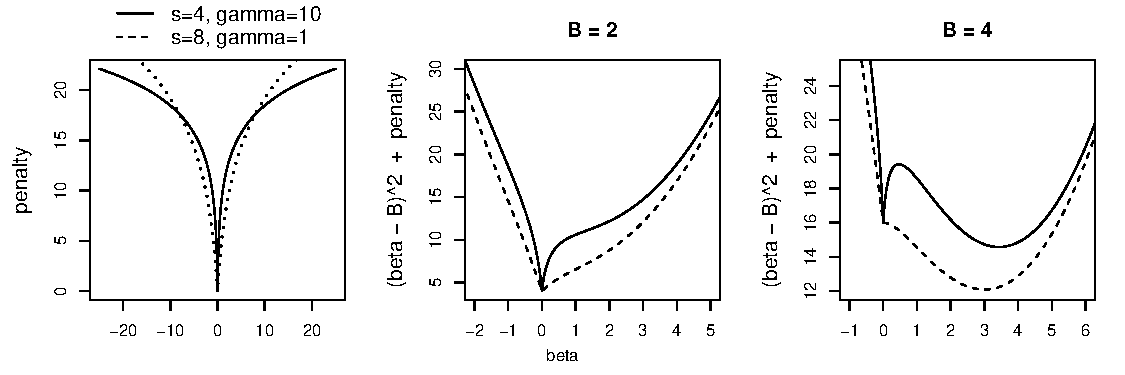
\includegraphics[width=6.4in]{solution}
\caption{\label{solution} Log penalties $c(\beta) = s\log(1 + \gamma|\beta|)$ 
and penalized objectives $(\beta-B)^2 + c(\beta)$.}
\end{figure}

\subsection{Concave cost functions and their implementation}
\label{concavecosts}

The dominant literature on diminishing bias estimation revolves around
{\it folded concave penalties}, such as SCAD 
\citep{fan_variable_2001} and MCP \citep{zhang_nearly_2010}.
These concave cost functions are purpose-built to avoid solution
discontinuity (see Section \ref{stability}). SCAD and MCP penalties are
implemented  in the {\tt ncvreg} {\sf R} package
\citep{breheny_coordinate_2011}, and elsewhere, but unfortunately the solvers
all require much more compute time than a standard lasso.  One run of SCAD via
{\tt ncvreg} for the simulation in Section \ref{sim} requires around 10
minutes, limiting the technology to small data analysis problems. This
slowness is due to the difficulty of concave minimization: finding global, or
even good local, minima is an extremely tough task.

One approach that does manage to quickly find good solutions  is the SparseNet
of \citet{mazumder_sparsenet_2011} which first fits a lasso path and, for each
$\lambda$ on this path, adapts coefficient estimates along a second path of
increasing concavity (analogous to increasing values of our $\gamma$). The
authors show that moving through a grid of both $\lambda$ and $\gamma$ in this
way helps to avoid minor modes and leads to faster convergence. An
implementation for the MCP penalty is in the {\tt sparsenet} package for {\sf
R}, and it is the best  software we've found for concave penalization.
Runtimes for {\tt sparsenet} and roughly equivalent loops of {\tt gamlr} over
multiple $\gamma$ are similar. The (significant) advantage of {\tt gamlr} is
that each different $\gamma$ specification can be run in parallel (or you can
just try one), while {\tt sparsenet} is inherently serial over dense $\gamma$
and $\lambda$ sequences.

\subsection{Concave penalization and weighted $L_1$ costs}
\label{lla}

Another relatively fast class of solvers for concave penalized estimators uses
local linear approximation \cite[LLA; e.g.,][]{candes_enhancing_2008}. LLA
replaces the concave cost function $c_j$  with its tangent at the current
estimate, $c_j'(\hat\beta_j)\beta_j$.  The objective is then just a weighted
$L_1$ penalized loss (solvable, say, as in Appendix \ref{implement}), and one
iterates between updating $c'(\hat\beta)$ and solving the implied $L_1$
penalized minimization problem. For example, LLA under the log penalty
 as in Section \ref{bayes} has $c'(\beta) = s \gamma / (1 + \gamma
|\beta|) = n\lambda/(1 + \gamma |\beta|)$, exactly our gamma lasso cost in
(\ref{l1pen}).


The LLA method  is simple and locally convergent, but  it can be
sensitive to initial starting location.  Consider approximating the log
penalized objectives of Figure \ref{solution} with LLA $l(\beta) +
c'(0)|\beta|$:  the approximation will minimize at $\beta=0$  until
$|l'(\beta)| > c'(0)$, even when the true objective $\beta\neq 0 $ local
minimum is much lower. Thus in a path estimation algorithm, LLA sticks at zero
until it jumps all the way out to near the MLE.

Despite this issue, \citet{zou_one-step_2008} present numerical and
theoretical evidence that  LLA does well in practice. Importantly, they
show that LLA does well even (or especially) if you {\it stop it after one
iteration}. This is an example of one-step estimation (OSE), a general
technique inspired by \cite{bickel_one-step_1975} that amounts to taking as
your estimator the first step of an iterative approximation to some objective.
Such early-stopping can be as good asymptotically as the full-step
solution {\it if} the initial estimates are good enough. OSE and similar
ideas have had a resurgence in the concave penalization literature recently,
motivated by the need for faster estimation algorithms.  OSE LLA requires only  convex weighted $L_1$ minimization.

\cite{fan_strong_2014} consider early-stopping of LLA
for folded concave penalization  and show that, under strong sparsity
assumptions about true $\bs{\beta}$ and given appropriate initial values, OSE
LLA is with high probability an oracle estimator.   Zhang (2010,2013)
\nocite{zhang_analysis_2010,zhang_multi-stage_2013} investigates  
`convex relaxation' iterations, where estimates under convex regularization
 are the basis for weights in a subsequent penalized objective.  He
shows that just one or two steps here is sufficient for obtaining oracle
support recovery properties under much weaker conditions than required by a
standard lasso.  \cite{wang_calibrating_2013} propose a two step algorithm
that feeds lasso coefficients into a linear approximation to folded concave
penalization.  They derive properties of entire regularization paths (e.g.,
guarantees that an oracle estimator is on the path) and construct a version of
the BIC for selection along these paths.


If one uses OSE LLA, or a two-step estimator starting from
$\bs{\hat\beta}=0$ as suggested in \cite{fan_strong_2014} and
\cite{wang_calibrating_2013}, the result {\it is just weighted $L_1$
minimization}. Thus OSE methods are  closely related to  the adaptive lasso
\citep[AL;][]{zou_adaptive_2006}, which does weighted $L_1$ minimization under
weights $\omega_j = 1/|\hat\beta^0_j|$, where $\hat\beta^0_j$ is an initial
guess at the coefficient value.  The original paper advocates using MLE
estimates for initial values, while
\cite{huang_adaptive_2008} suggest using marginal regression coefficients
$\hat\beta^0_j = \mr{cor}(\bm{x}_j,\bm{y})$ and show that this can provide oracle
properties in the  $p>n$ setting (we include marginal AL in our study of
Section \ref{sim}).  Like GL, AL provides
diminishing bias penalization without solving for an explicit concave penalty.

Each segment of our gamma lasso path is also a one-step estimator, for log
penalized objectives starting from the estimates at the previous segment.  And
since path estimation relies on $\bs{\hat\beta}^{t-1}$ being close to
$\bs{\hat\beta}^{t}$, it seems a natural partner for OSE. All of these methods
-- GL, LLA OSE, AL -- differ only in how the weights are
constructed.  Regardless of which you prefer, weighted $L_1$ penalties are
likely to play a central role in diminishing bias penalization whenever the
dataset is too large for use of exact concave penalty solvers.

\section{Comparison to $L_0$ penalized estimation}
\label{theory}

We are interested in $L_1$ penalization with data-dependent weights as a way
to obtain fits that are as sparse as possible without compromising predictive
ability.  We do not assume a true sparse model, so that our
benchmark is estimation under $L_0$ costs $c_j(\beta_j) = \ds{1}_{\{\beta_j\neq0\}}$.   Since $L_0$ penalized minimization
is an NP-hard problem, it is practically impossible to find a
global solution.  However, in this section we present finite sample bounds on
the distances -- in prediction and on coefficients -- between  $L_0$  and weighted
$L_1$ penalized estimation.  This comparison yields simple
relationships that make no assumptions about the underlying data model.
Moreover, when we do make standard assumptions about the data generating
process, we are able to quantify distance between weighted $L_1$ estimates and
a theoretically optimal $L_0$ penalized estimator.


\subsection{Sparse Approximation for Prediction}

 For any support subset $S \subset \{1\ldots p\}$ with cardinality $|S|=s$ and
complement $S^c = \{1\ldots p\}\setminus S$, denote vectors restricted to $S$
as $\bm{\beta}_S = [\beta_j:j\in S]'$, matrices as $\bm{X}_S$, etc.  Use
$\bs{\beta}^S$ to denote the coefficients for ordinary
least-squares (OLS) restricted to $S$: that is, $\bs{\beta}^S_S =
(\bm{X}_S'\bm{X}_S)^{-1}\bm{X}_S'\bm{y}$ and $\beta^{S}_j = 0~\forall~j\notin
S$.  Moreover, $\bm{e}^S = \bm{y}-\bm{X}\bs{\beta}^S =
(\bm{I}-\bm{H}^S)\bm{y}$ are residuals and $\bm{H}^S =
\bm{X}_S(\bm{X}_S'\bm{X}_S)^{-1}\bm{X}_S'$ the hat (projection) matrix from OLS restricted to $S$.  We suppress intercepts throughout, and use $|\cdot|$ and $\|\cdot\|$ applied to vectors as the $L_1$ and $L_2$ norms, respectively.

We'll use the following simple result for stagewise regression -- iterative fitting of new covariates to the residuals of an existing linear model (as in, e.g., \citealt{goldberger_stepwise_1961}). 
\begin{lemma}\label{SSElemma}
Say $\mr{MSE}_S = \|\bm{X}\bs{\beta}^S-\bm{y}\|^2/n$ and 
$\mr{cov}(\bs{x}_j,\bm{e}^S) = \bs{x}_j'(\bm{y}-\bm{X}\bs{\beta}^S)/n$ are sample variance and covariances.  Then for any $j \in 1\ldots p$, 
\[
\mr{cov}^2(\bs{x}_j,\bm{e}^S) \leq \mr{MSE}_S - \mr{MSE}_{S\cup j}
\]
\end{lemma}
\begin{proof}
From the well-known property on the correlation coefficient ($R^2$) for linear models,   
in-sample correlation and variances are such that
\[
\frac{\mr{cov}^2(\bs{x}_j,\bm{e}^S)}{\mr{var}(\bs{x}_j)\mr{var}(\bm{e}^S)} = 1 - \frac{\mr{var}(\bm{e}^S-\tilde\beta_j\bs{x}_j)}{\mr{var}(\bm{e}^S)}
\]
where $\tilde\beta_j = \bs{x}_j'\bm{e}^S/(\bs{x}_j'\bs{x}_j)$ is the stagewise coefficient estimate.  Since $\mr{var}(\bs{x}_j)=1$, multiplying everything by $\mr{var}(\bm{e}^S)$ yields $\mr{cov}^2(\bs{x}_j,\bm{e}^S) =
\mr{var}(\bm{e}^S) - \mr{var}(\bm{e}^S-\tilde\beta_j\bs{x}_j)
\leq \mr{var}(\bm{e}^S) - \mr{var}(\bm{e}^{S\cup j})$.
The last inequality holds because $\bm{e}^{S\cup j}$, residuals from OLS on $\bm{X}_{S\cup j}$, have the smallest-possible sum of squares for that set of covariates.  With $\mr{var}(\bm{e}^S) = \mr{MSE}_S$, etc, we are done.
\end{proof}

In addition, we need to define {\it restricted eigenvalues} (RE) on the gram matrix $\bm{X}'\bm{X}/n$.  
\begin{definition}\label{redef}
The restricted eigenvalue is
$
\phi^2(L,S) = \min_{\{\bm{v}: \bm{v}\neq \bm{0},~|\bm{v}_{S^c}| \leq L\sqrt{s}\|\bm{v}_S\|\}}\frac{\|\bm{X}\bm{v}\|^2}{n\|\bm{v}\|^2}$.
\end{definition}
\noindent The specific RE in Definition (\ref{redef}) matches the `adaptive restricted eigenvalues' of \cite{buhlmann_statistics_2011}.  These and related RE quantities are common in prediction and estimation results for both $L_1$ and concave penalization schemes.  See the remarks for more detail.

Finally, our result derives a bound on the distance between prediction rules based on $L_0$ and weighted $L_1$ penalized estimation.  Intercepts are suppressed for simplicity.
\begin{theorem} \label{sparseapprox}  Consider squared-error loss $l(\bs{\beta}) =
\frac{1}{2}\|\bm{X}\bs{\beta}-\bm{y}\|^2$, and suppose $\bs{\beta}^{\nu}$ minimizes the $L_0$ penalized objective $l(\bs{\beta}) + n\nu\sum_{j=1}^p\ds{1}_{\{\beta_j\neq0\}}$ with $\bs{\beta}^\nu = \bs{\beta}^S$ and $|S|=s<n$.   
Write $\bs{\hat\beta}$ as solution to the weighted $L_1$ minimization $l(\bs{\beta}) + n\lambda\sum_j\omega_j|\beta_j|$. 

Then  
$\omega^{\mr{min}}_{S^c}\lambda > \sqrt{2\nu}$ while $\phi^2(L,S) > 0$ implies
\begin{equation} \label{sparseineq}
\frac{\|\bm{X}(\bs{\hat\beta}-\bs{\beta}^\nu)\|^2}{n}\leq
\frac{4\lambda^2 \|\bs{\omega}_S\|^2}{\phi^2(L, S)}
\end{equation} 
with the restricted eigenvalue defined for 
 $L = \frac{\|\bs{\omega}_S\|}{\sqrt{s}}\left(\omega^{\mr{min}}_{S^c}-\sqrt{2\nu}/\lambda\right)^{-1}$.
\end{theorem}

\begin{proof}
From the definitions of $\bs{\hat\beta}$ and $\bs{\beta}^\nu = \bs{\beta}^S$, 
\begin{align}\label{predconv}
\frac{1}{2}\|\bm{X}\bs{\hat \beta}-\bm{y}\|^2 + & n\lambda\sum_j\omega_j|\hat\beta_j|  ~~=~~ \frac{1}{2}\|\bm{X}(\bs{\hat\beta}-\bs{\beta}^\nu)\|^2 + \frac{1}{2}\|\bm{e}^S\|^2 - \bm{\hat y}'\bm{e}^S+ n\lambda\sum_j\omega_j|\hat\beta_j|\\
&~~~~~~~~~~~~~~~~~~~ \leq~~ \frac{1}{2}\|\bm{X}\bs{\beta}^\nu-\bm{y}\|^2 + n\lambda\sum_j\omega_j|\beta^\nu_j| ~~=~~ \frac{1}{2}\|\bm{e}^S\|^2 + n\lambda\sum_{j\in S}\omega_j|\beta^S_j|\notag
\end{align}
  Since $\bm{\hat y}'\bm{e}^S = \bm{\hat y}'(\bm{I}-\bm{H}^S)\bm{y} =
\bs{\hat\beta}'\bm{X}'(\bm{y}-\bm{X}\bs{\beta}^\nu) = 
\sum_{j\in S^c} \hat\beta_j\bs{x}_j'(\bm{y}-\bm{X}\bs{\beta}^\nu)
$,
 we can apply Lemma \ref{SSElemma} followed by $\bs{\beta}^\nu$ being optimal under $L_0$ penalty $\nu$ to get 
\begin{equation} \label{L0ineq}
\left(\frac{\bs{x}_j'(\bm{y}-\bm{X}\bs{\beta}^\nu)}{n}\right)^2
\leq \mr{MSE}_S - \mr{MSE}_{S\cup j} < 2\nu ~~~\forall~j
\end{equation}
so that $|\bm{\hat y}'\bm{e}^S| = |\bs{\hat\beta}_{S^c}\bm{X}_{S^c}'(\bm{y}-\bm{X}\bs{\beta}^\nu)| < n\sqrt{2\nu}|\bs{\hat\beta}_{S^c}|$.  Applying this inside (\ref{predconv}),
\begin{align}\label{predconvineq}
\frac{1}{2}\|\bm{X}(\bs{\hat\beta}-\bs{\beta}^\nu)\|^2
  + n\left(\omega^{\mr{min}}_{S^c}\lambda-\sqrt{2\nu}\right)|\bs{\hat\beta}_{S^c}|
  &~\leq~ n\lambda\sum_{j\in S}\omega_j|\hat\beta_{j}-\beta^\nu_j|
  ~\leq~ n\lambda\|\bs{\omega}_S\|\|\bs{\hat\beta}_{S}-\bs{\beta}^\nu_S\|.
\end{align}
Given $\omega^{\mr{min}}_{S^c}\lambda > \sqrt{2\nu}$,
difference $\bs{\hat\beta}-\bs{\beta}^\nu$ is in the RE support for 
$L=\frac{\|\bs{\omega}_S\|}{\sqrt{s}}(\omega^{\mr{min}}_{S^c}-\sqrt{2\nu}/\lambda)^{-1}$ and thus $\|\bs{\hat\beta}_{S}-\bs{\beta}^\nu_S\| \leq \|\bm{X}(\bs{\hat\beta}-\bs{\beta}^\nu)/\sqrt{n}\|/\phi(L,S)$.  Finally, applying this inside (\ref{predconvineq}) yields
\begin{align}
\frac{1}{2}\|\bm{X}(\bs{\hat\beta}-\bs{\beta}^\nu)\|^2
  &~\leq~ \frac{\sqrt{n}\lambda\|\bs{\omega}_S\|\|\bm{X}(\bs{\hat\beta}-\bs{\beta}^\nu)\|}
  {\phi(L, S)}.
\end{align}
Dividing each side by $\sqrt{n}\|\bm{X}(\bs{\hat\beta}-\bs{\beta}^\nu)\|/2$ and squaring gives the result.
\end{proof}

\noindent {\bf Remarks}

\vskip .25cm
\noindent $\bullet$~~  This is finite sample exact and completely non-parametric -- it makes no reference to the true distribution of $\bm{y}\mid \bm{X}$.  Indeed, if we make such assumptions, Theorem \ref{sparseapprox} provides bounds on the distance between a weighted lasso and optimal prediction.  The next remark is an example.

\vskip .25cm
\noindent $\bullet$~~ If we assume that $\bm{y} \sim
(\bs{\eta},\sigma^2\bm{I})$ --  $y_i$ independent with mean $\mu_i$
and shared variance $\sigma^2$ -- then the $C_p$ formula of  
\citep{mallows_comments_1973} provides 
$\mr{MSE}_S + 2s\sigma^2/n$ as an unbiased estimate of residual variance.
Following \cite{efron_estimation_2004}, this implies $\nu = \sigma^2/n$ is the optimal $L_0$ penalty for minimizing prediction error.  
Theorem (\ref{sparseapprox}) applies directly,  with $L = \frac{\|\bs{\omega}_S\|}{\sqrt{s}}\left(\omega^{\mr{min}}_{S^c}- \sqrt{2}\sigma/(\lambda\sqrt{n})\right)^{-1}$, to give a bound on the distance between weighted $L_1$ estimation and $C_p$-optimal prediction.\footnote{We work with
$C_p$ here, rather than $AIC$ or $AICc$, since $C_p$ is conveniently defined
the scale of squared errors.} Note that, since the condition on minimum $S^c$ weights has become
$\omega^{\mr{min}}_{S^c} > (\sigma/\lambda)\sqrt{2/n}$, comparison to $C_p$ suggests we can use larger $\gamma$ (faster diminishing bias) with large $n$ or small $\sigma$.


\vskip .25cm
\noindent $\bullet$~~  Plausibility of the restricted eigenvale assumption $\phi(L,S) > 0$ depends  upon $L$.  It is less restrictive if we can reduce $\|\bs{\omega}_S\|$ without making $\omega^{\mr{min}}_{S_c}$ small.  For example, the next sub-section suggests using large $\gamma$ so long as $\lambda$ is big enough to avoid false discovery. \cite{raskutti_restricted_2010} show that similar conditions hold given  $\omega^{\mr{min}}_{S_c}=1$ with high probability for $\bm{X}$ drawn from a broad class of Gaussian distributions.  \cite{bickel_simultaneous_2009} provide a nice overview of sufficient conditions, and \cite{buhlmann_statistics_2011} have extensive discussion and examples.


\subsection{False Discovery Control}

A common goal in high-dimensional estimation is  support recovery -- having the set $\{j: \hat\beta_j \neq 0\} = \{j: \beta_j \neq 0\}$ for some `true' $\bs{\beta}$.
For standard lasso estimated $\bs{\hat\beta}$, many authors have shown \citep[e.g.,][]{buhlmann_statistics_2011,zou_adaptive_2006} that to get exact support recovery asymptotically or with high probability requires an {\it irrepresentability condition} which limits the size of least-squares projections from `true support' onto spurious covariates.  
\begin{definition} 
The $(\theta,S,\bm{v})$-irrepresentable condition for $\theta\in[0,1]$ and $\bm{v}\in \ds{R}^s$ holds that, 
\begin{equation}\label{irrep}
|\bs{x}_j'\bm{X}_S(\bm{X}_S'\bm{X}_S)^{-1}\bm{v}| \leq \theta ~~\forall~j\notin S
\end{equation}
\end{definition}
\noindent This is often presented with $\bm{v}=\bm{1}$.\footnote{\cite{wainwright_sharp_2009} shows that (\ref{irrep}) with $\theta=1$, $\bm{v}=\bm{1}$ is necessary for lasso sign recovery in the {\it noiseless} setting.} It
can be a strict design restriction; for example,
\citet{buhlmann_statistics_2011} show a single variable that is
highly correlated with many columns of $\bm{X}_S$ leading to failure. Much
of the literature on concave penalization has focused on achieving
support recovery {\it without} such conditions; see, e.g.,
\cite{fan_strong_2014} for a recent overview.  
Our results will require irrepresentable conditions with $\bm{v} =
\bs{\omega}_S$, which becomes less restrictive as one is able to shrink
weights $\omega_j$ for $j\in S$.  See the remarks for more discussion.

Our comparison of interest is between $\hat S = \{j:
\hat\beta_j \neq 0\}$, for $\bs{\hat\beta}$ from weighted $L_1$ penalized
estimation, and $S = \{j:
\beta^\nu_j \neq 0\}$ for $\bs{\beta}^\nu$ the $L_0$ penalized estimator from
Theorem \ref{sparseapprox}. Whether looking to an $L_0$ oracle or a sparse
truth, our experience is that exact support recovery does not occur in
practice   (e.g., see the simulation in Section \ref{sim}).  Thus, we instead 
focus on ability of the weighted lasso to minimize {\it false discoveries}:
$\hat\beta_j
\neq 0$ when $\beta^\nu_j=0$.  In particular, we describe how far along the regularization path one may expect to avoid any false discovery.


\begin{theorem}
Consider the setting of Theorem \ref{sparseapprox}, but where $\bs{\hat\beta}
= \bs{\hat \beta}_t$ is now the solution at segment `$t$' of a gamma lasso path,
and say that $\hat S_{t} = \{j:\hat\beta^{t}_j\neq 0\}$.  

If $\hat S_{t-1}
\cap S^c = \varnothing$ and $\lambda_t > \sqrt{2\nu}$ then
\begin{equation}\label{falsepos}
\|\bm{X}_{S^c}'\bm{X}_S(\bm{X}_S'\bm{X}_S)^{-1}\bs{\omega}^t_S\|_{\infty} \leq 1 - \frac{\sqrt{2\nu}}{\lambda_t} ~~\Rightarrow~~\hat S_{t} \cap S^c = \varnothing.
\end{equation}
\end{theorem}
\noindent The result follows directly from the sign recovery lemma in Appendix
\ref{extraproof}. 

\vskip .25cm
\noindent {\bf Remarks}
\vskip .25cm
\noindent $\bullet$~~ 
The results uses $\hat S_{t-1} \cap S^c = \varnothing \Rightarrow \omega_{S^c}^{t~\mr{min}} = 1$ for the GL algorithm.  So long as $\lambda_t$ is large enough, (\ref{falsepos}) suggests that  big $\gamma$ (for fast diminishing $\omega_j$) will help control false discovery.  Of course, the momment $\hat S_{t-1} \cap S^c \neq \varnothing$,  a large $\gamma$ allows spurious covariates to enter with very little shrinkage and can move the fit arbitratily far away from $L_0$-optimal support.

\vskip .25cm
\noindent $\bullet$~~ 
From Theorem 7.4 in \cite{buhlmann_statistics_2011}, 
the irrepresentability condition holds with 
$|\bs{x}_j'\bm{X}_S(\bm{X}_S'\bm{X}_S)^{-1}\bs{\omega}_S|
\leq \frac{\|\bs{\omega}_S\|}{\sqrt{s}}\theta_{\mr{adap}}(S)$ where $\theta_{\mr{adap}}(S)$ is their `adaptive restricted regression' coefficient.  Of interest here, they show that $\theta_{\mr{adap}}(S) \leq \sqrt{s}/\Lambda_{\mr{min}}(S)$ where $\Lambda_{\mr{min}}(S)$ is the minimum eigenvalue of $\bm{X}_S'\bm{X}_S/n$.  Thus, $(i)$ can be replaced by the restriction $\Lambda_{\mr{min}}(S) \geq \|\bs{\omega}_S\|(1 - \sqrt{2\nu}/(\omega_{S^c}^{\mr{min}}\lambda))^{-1} = \sqrt{s}L$, with $L$ from Theorem \ref{sparseapprox}, and small values for $L$ appear key in both predictive performance and support recovery.

\vskip .25cm
\noindent $\bullet$~~ Without irrepresentability,  limits on false discovery are more pessimistic.  Convergence
conditions imply that for $j \in S^c \cap \hat S$ we have
$n\lambda \omega_j = |\bs{x}_j'(\bm{X}\bs{\hat\beta}-\bm{y})| \leq
|\bs{x}_j'\bm{X}(\bs{\hat\beta}-\bs{\beta}^\nu)| + |\bs{x}_j'\bm{e}^S| \leq
n\left(2\|\bs{\omega}_S\|/\phi(L,S) + \sqrt{2\nu}/\lambda\right) ~\forall~j$. 
Dividing by $n\lambda\omega_j$ and counting yields
\begin{equation}\label{pessimism}
|S^c \cap \hat S| \leq \left|\frac{1}{\bs{\omega}_{S^c \cap \hat S}}\right|
\left(\frac{2\|\omega_S\|}{\phi(L,S)} + \frac{\sqrt{2\nu}}{\lambda}\right)
\end{equation}
Without the ability to
make $\omega_j$ very big for $j \in S^c$ (e.g., as in a thresholding procedure
like that of \citealt{zhou_thresholding_2009}), the result in (\ref{pessimism}) has little to say about false discovery control.


\section{Stability}
\label{stability}

The benefits of diminishing bias come at a price: the negative log posterior
can be concave.  This can lead to large changes in fit from small change in
{\it either} data $\bm{y}$ or penalty size $\lambda$.  For example,  the
minimizer of the solid line of the right panel in Figure \ref{solution} will
jump from 0 to 3.5 depending upon small jitter either to data $B$ or cost
$\gamma s$.

Estimators that make large changes under small
data jitter are {\it instable}.  This hurts predictive performance by
increasing predictor variance, it precludes estimation of model complexity as
in Section \ref{dof}, and
\citet{breiman_heuristics_1996} argues that variability of model choice
explodes if the candidate fits are themselves instable. From another
perspective, a fit that is {\it sensitive} to specification is unreliable when
there is model uncertainty. And if $\bs{\hat\beta}$ jump along the
regularization path -- that is, if the paths are non-smooth functions of
$\lambda$ -- then $\bs{\hat\beta}^{t-1}$ is no longer a good hot-start for
$\bs{\hat\beta}^t$.

% The rest of this section connects solution discontinuity to our Bayesian model, before looking at each of stability under data jitter and  sensitivity to penalty size.

\subsection{Stability and the Bayesian model prior}

For orthogonal inputs, the penalized objective becomes concave only if
negative log likelihood coordinate curvature $h_j = \partial^2 l(\bs{\beta})/\partial
\beta_j^2$, which does not depend upon $y$ for exponential families, is less
than the absolute value of the curvature on the cost function for $\beta_j$.
Absolute curvature for the log penalty is $s\gamma^2$ at the origin, and less
elsewhere, such that  the objective in (\ref{logobj}) is guaranteed convex if
$s\gamma^2 < h_j$.  For correlated inputs, one has objective convexity if the
minimum eigenvalue of $\bm{H}$, the Hessian matrix of second derivatives of
$l(\bs{\beta})$, is greater than $s\gamma^2$.\footnote{ \noindent If $\nu$ is an
eigenvalue of $\bm{H}$, then $(\bm{H} -
\nu \bm{I})\bm{v} = 0$ for some nonzero $\bm{v}$; the negative log posterior
Hessian at zero is $\bm{H} - s\gamma^2\bm{I}$ and $(\bm{H} - s\gamma^2\bm{I} + s\gamma^2\bm{I} -
\nu \bm{I})\bm{v} = 0$ so that 
$\nu - s\gamma^2$ is an eigenvalue of the minimization objective.}

Recognizing $\gamma^2 s$ as the variance of a $\mr{Ga}(s,\gamma^{-1})$
distribution, the above can  interpreted in the context of our Bayesian model
from Section \ref{bayes}:  the joint MAP is continuous  if the prior variance
on each $\tau_j$ coefficient scale is less than the minimum eigenvalue of the
likelihood information matrix $\bm{H}$. For Gaussian regression with
standardized orthogonal covariates, $h_j = \sum_i x_{ij}^2 = n$ and we get a
simple rule: the joint MAP is continuous  if prior variance on each $\tau_j$  is
less than the number of observations.  For logistic regression you need
$\mr{var}(\tau_j) < n/4$.


\subsection{Lipshitz continuity}

One possible definition of stability requires Lipschitz continuity. Say
$\hat\beta(\bm{y})$ is our implicit estimation function. Then $\hat\beta$ is
Lipschitz continuous if  $ \|\hat\beta(\bm{y}_1)-\hat\beta(\bm{y}_2)| \leq
L\|\bm{y}_1-\bm{y}_2\| $ for some finite constant $L$ on all possible
$\bm{y}_1,\bm{y}_2$. This is necessary for, e.g., our degrees of freedom
estimator in Section \ref{dof}.  Many popular concave cost functions, such as
the SCAD and MC+, have been engineered to be Lipschitz continuous.
\cite{zou_one-step_2008} show that OSE LLA solutions have this property even
if the target objective does not.

More generally, since $L_1$ penalized least-squares estimators are Lipschitz continuous \cite[][]{zou_degrees_2007}, versions that use data-dependent penalty weighting will also be continuous so long as the weights are themselves finite and continuous functions of $\bm{y}$.\footnote{Holds also for generalized linear models under conditions that make maximum likelihood estimators continuous.}  This can be used to establish continuity of, e.g., AL with inverse weights set as marginal correlations or through a preliminary lasso run.  It also rules out continuity whenever weights are derived from hard-thresholding, such as in the thresholded lasso studied by \cite{van_de_geer_adaptive_2011}.
For the gamma lasso, we are able to establish continuity of the entire regularization path.

\begin{prop} For $\gamma<\infty$ the least-squares gamma lasso path is Lipschitz continuous. \end{prop} 
\begin{proof}
From the above discussion, we need to establish continuity of the weights.  At $\lambda_1$ and $\lambda_2$, the weights are always all one.  And if $\bs{\beta}^{t}$ are Lipschitz continuous,  then so are $\bs{\omega}^{t+1}$ for all $\gamma<0$ and thus $\bs{\beta}^{t+1}$ is Lipschitz continuous.  By induction the entire path is continuous.
\end{proof}


\subsection{Practical Stability}

A regularization path can be Lipschitz continuous but still overly sensitive to data jitter and penalty size.  The most obvious effect is computational:  when solutions change too quickly along the path, you lose the benefit of hot-starts and computation time blows up. As an illustration, Figure \ref{nhltime} shows timings growing rapidly with large $\gamma$ for the hockey data  of Section \ref{nhl}, even though all of these specifications are theoretically stable.

\begin{figure}[bht]
\vskip -.5cm
\centering
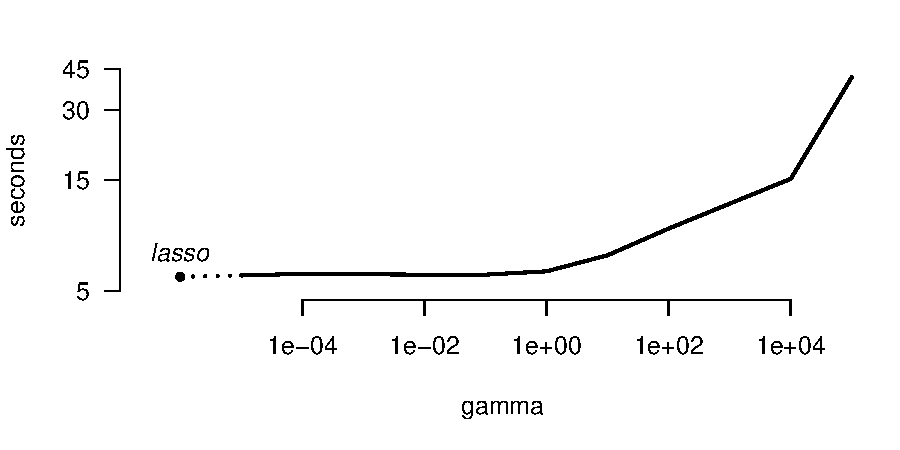
\includegraphics[width=5in]{nhl_time}
\vskip -.25cm
\caption{\label{nhltime} 
Timings for the hockey data path fits of Section \ref{nhl}
on a length-100 grid with $\lambda^{100} = 0.01\lambda^1$. }
\vskip -.25cm
\end{figure}


\section{Degrees of freedom}
\label{dof}

A predictor's degrees of freedom ($df$) determines its tendency to over or
under fit, and is a key input for model selection. In an unpenalized linear
model, $df$ is just the number of coefficients.  More generally, for $\bm{y} \sim (\bs{\eta},\sigma^2\bm{I})$
we define $df = \sigma^{-2} \sum_i \mr{cov}(\hat y_i, y_i)$ where $\hat y_i$
is the prediction rule for observation $y_i$ \citep[e.g.][]{efron_least_2004}. Given an estimator
that is Lipschitz continuous with respect to $\bm{y}$, as in Section
\ref{stability}, the SURE framework of \cite{stein_estimation_1981} applies
and we get a more workable version of this definition:  $df =
\ds{E}\left[\sum_i \partial \hat y_i/\partial y_i\right]$.

Consider  a single coefficient $\beta$ estimated via least-squares
under $L_1$ penalty $\tau$.   Write gradient at zero $g = -\sum_i
x_iy_i$ and curvature $h = \sum_i x_i^2$ and set $\varsigma = -{\tt sign}(g)$.
The prediction rule is $\hat y =
x(\varsigma/h)(|g|-\tau)_+$ with  derivative $\partial \hat y/\partial y =
x_i^2/h \ds{1}_{[|g|<\tau]}$, yielding 
$df = \ds{E}\left[ \ds{1}_{[|g|<\tau]} \right]$.   For many orthogonal
covariates, we get $\hat y = \sum_j x_j(\varsigma_j/h_j)(|g_j|-\tau_j)_+$ and
\begin{equation} \label{sure} df = \sum_j
\ds{E}\left[ \ds{1}_{[|g_j|<\tau_j]} \right].
\end{equation}
\cite{zou_degrees_2007} plug sample gradients into (\ref{sure}) to derive
$\hat{df} = \sum_j \ds{1}_{|g_j| < \tau_j} = \sum \ds{1}_{|\hat\beta_j| \neq 0} = \hat p$, the number of
nonzero  coefficients, as an unbiased estimator of lasso
degrees of freedom.


We'll use the same tactic of plugging-in observed gradient.  However, for the
GL algorithm with $\gamma>0$ each $\tau_j$ is a function of $\bm{y}$.
Moreover, estimated $\hat\tau_j$ have been optimized to fit the data and
plugging them into (\ref{sure}) yields a biased (low) estimate of $df$.
Instead, we take advantage of the Bayesian  hierarchical model of Section
\ref{bayes} and average (\ref{sure}) over the $\mr{Ga}(s,1/\gamma)$ prior on
$\tau_j$. This implies the {\it gamma lasso estimator for degrees of freedom}
\footnote{The number of unpenalized coefficients (e.g.,~1 for
$\alpha$) is always added to this to get total $df$.} 
\begin{equation}
\label{edf} df^t = \sum_j \mr{Ga}(|g_{j}|;~ n\lambda^t/(\gamma\phi),
1/\gamma), \end{equation} where $\mr{Ga}$ is the Gamma distribution
function. Note that $\lim_{\gamma \to 0} df^t = \hat
p^t$ and  $\lim_{\gamma \to \infty} df^t= p$.

As a Bayesian prior estimate of a frequentist statistic, (\ref{edf}) is a
clearly heuristic formula.  There are also a number of approximations
necessary in application.  Gaussian regression requires $\phi
\approx \hat\sigma^{2t} = \sum_i (y_i - \hat y^t_i)^2/n$, which biases
 $df^t$ upwards from truth for over-fit models and downwards with
under-fit.   In the non-orthogonal case, where $g_{j} = g_j(0)$ becomes a
function of all of the elements of $\bs{\beta}$, we plug in the most recent
$g_j$ at which $\hat\beta^t_j=0$:  this
requires no extra computation and has the advantage of maintaining $df =
\hat p^t$ for $\gamma = 0$.  And for non-Gaussian models (e.g.,
in Section \ref{nhl}), we apply (\ref{edf}) directly despite its
motivation from squared errors.

Despite these many compromises, we have found that (\ref{edf}) works remarkably
well in both simulation and real data examples.  When used as an input to
information criteria, as in the next section, it allows those criteria to
perform as well or better than nonparametric cross-validation.

\section{Selection}
\label{selection}


The dominant model selection paradigm in Big data analysis attempts to choose
 a model that performs well in predicting new data. Even if one is primarily
 interest in support recovery, authors such as \cite{hastie_elements_2009}
 recommend predictive performance optimization accompanied by a hedge towards
 simplicity (i.e., the 1se rule of Section \ref{cv}).  This focus on
 prediction is in part due to other tools (e.g., hypothesis testing) not
 scaling well with model dimension.  But in any case, it seems reasonable to
 avoid models that do a very poor job in prediction.

`Good prediction' can be measured in a variety of ways.  A common and coherent framework is to consider minimizing Kullback-Leibler (KL) divergence.  Say $g(\bm{y})$ is the true data generating process, and $f(\bm{y}; \bs{\eta},\phi)$ is the parametric density under study, which we suppose here is a natural exponential family  with $\ds{E}[\bm{y}]=\bs{\eta}$ and dispersion $\phi$. Then we wish to minimize
\begin{equation}
\mr{KL}(\bs{\eta},\phi) = \ds{E}_g \log g(\bm{y}) - \ds{E}_g \log f(\bm{y}; \bs{\eta},\phi),
\end{equation}
the expected difference between log true density and our parametric approximation.  Since $\ds{E}_g \log g(\bm{y})$ is constant, this leads one to minimize 
$Q(\bs{\eta},\phi) = -\ds{E}_g \log f(\bm{y}; \bs{\eta},\phi)$, the expected negative log likelihood.   There is no requirement that $g$ is a member of the family defined by $f$.

If parameters are to be estimated as $[\bs{\eta}_{\bm{y}},\phi_{\bm{y}}]$, functions of random sample $\bm{y} \sim g$, then $Q(\bs{\eta}_{\bm{y}},\phi_{\bm{y}})$ is itself a random variable and one chooses estimators to minimize its expectation.  {\it Crucially, we imagine a double-sample expectation}, where the minimization objective is
\begin{equation}\label{dualexpect}
\ds{E}_{\bm{y}|g} \ds{E}_{\bm{\tilde y}|g} \log f(\bm{\tilde y}; \bs{\eta}_{\bm{y}},\phi_{\bm{y}}).
\end{equation}
The notation here indicates that inner and outer expectations are based on two {\it independent} random samples from $g$: $\bm{y}$ for training, upon which $\bs{\eta}_{\bm{y}},\phi_{\bm{y}}$ are calculated, and $\bm{\tilde y}$ for validation.  

The remainder of this section outlines two strategies for minimization of (\ref{dualexpect}).  The first, cross-validation, performs a Monte Carlo experiment that mimics double expectation.  The second set of methods, information criteria, attempt to approximate (\ref{dualexpect}) analytically via the observed likelihood and a complexity penalty that depends upon the degrees of freedom.

\subsection{Cross validation}
\label{cv}

$K$-fold cross-validation \cite[CV; see][for an
overview]{efron_estimation_2004} estimates the double expectation in
(\ref{dualexpect}) through a simple experiment: split the sample $\mc{S} =
\{\bm{x}_i,y_i\}_{i=1}^n$ into $K$  disjoint subsets (folds) $\mc{S}_k$,
and $K$ times fit a regularization path given $\mc{S} \setminus \mc{S}_k$ and
use this to predict on $\mc{S}_k$.  This yields $K$  realizations of
`out-of-sample' (OOS) deviance, and you averaged across folds to get an
estimate for (\ref{dualexpect}) along the along the regularization path. One then selects $\lambda$ according to some criterion and re-fits the
model on the entire dataset under this penalty.  The usual rules are either
CV.min, choose the $\lambda$ with minimum average OOS error, or
CV.1se, choose the largest $\lambda$ with mean OOS error no more than
1 standard error away from the minimum. 

CV is super useful, and some form of it features in most applications, but it
does have some weaknesses. If a single fit is expensive then doing it $K$
times will be impractical.  More subtly, truly Big data are distributed: they
are too large to store on a single machine. Algorithms can be designed to work
in parallel on subsets
\citep[e.g.,][]{taddy_distributed_2013}, but a bottleneck
results if you need to communicate across machines for OOS experimentation.
Finally, large organizations may wish to avoid the
Monte Carlo error of CV -- they'll want the same answer every time.  Thus it
is useful to have an analytic estimator for (\ref{dualexpect}) that requires only  a single model fit.


\subsection{Information Criteria: AIC and AICc}


Information criteria (IC) are analytic approximations to metrics like (\ref{dualexpect}).  They take the form
\begin{equation}\label{ic}
 -2\log f(\bm{y}; \bs{\eta}_{\bm{y}},\phi_{\bm{y}}) + c(df)
 \end{equation} 
where $c(df)$ is a penalty on the degrees of freedom used in $\bs{\eta}_{\bm{y}}$.
 We can plug-in the $df^t$ degrees of
freedom heuristic from (\ref{edf}) here, and the IC-selected model is that
which minimizes (\ref{ic}).

The commonly applied AIC uses $c(df)=2df$ and is derived as an asymptotic approximation to (\ref{dualexpect}) in 
\cite{akaike_information_1973}.  However, our experience (e.g., see Section
\ref{sim}) is that AIC selects over-fit models when applied to high dimensional
problems.  This is because the approximation upon which it is based
is valid only for large $n/df$ \citep{burnham_model_2002}.  A `corrected' AICc
for finite $n/df$ is derived in
\cite{hurvich_regression_1989}, and \citet{flynn_efficiency_2013} study its
application to penalized deviance estimation.
\begin{equation}
\text{AICc:}~~~-2\log f(\bm{y}; \bs{\eta}_{\bm{y}},\phi_{\bm{y}}) + 2df\frac{n}{n-df-1}.
\end{equation}
The correction multiplier is $n/(n-df-1)$, and AICc approaches standard AIC if $n\gg df$.  We find massive improvements from this correction, and in our simulations (and other experience) AICc can match or exceed the  performance of CV-based selection.  

Since the AICc plays a central role in our applied work, we present below an informal derivation based on the Mallows $C_p$ formula.  The goal here is to make the result as intuitive as possible.  See \cite{claeskens_model_2008} for a more traditional derivation and full theoretical review of information criteria, and refer to \citet{flynn_efficiency_2013} for results extending to generalized linear models (which we take for granted in the hockey application of Section \ref{nhl}). 

\subsubsection{Derivation of AIC and AICc}

Consider a Gaussian regression model where $\bs{\eta}_\bm{y}$ is an estimate
for $\bs{\eta} = \ds{E}\bm{y}$ using $df$ degrees of freedom, and set $\phi_\bm{y} =
\sigma^2_{\bm{y}} = \sum_i (y_i - \eta_{\bm{y}i})^2/n$. We'll derive
\begin{equation}\label{aiccapprox}
df\frac{n}{n-df-1}  \approx \ds{E}_{\bm{y}|g}\left[\log f(\bm{y}; \bs{\eta}_{\bm{y}},\phi_{\bm{y}}) - \ds{E}_{\bm{\tilde y}|g} \log f(\bm{\tilde y}; \bs{\eta}_{\bm{y}},\phi_{\bm{y}})
\right],
\end{equation}
such that AICc's complexity penalty is the expected bias that results from taking the fitted log likelihood as an estimate for (\ref{dualexpect}).  First, by cancellation the inner term of (\ref{aiccapprox}) simplifies as 
\begin{equation}
\log f(\bm{y}; \bs{\eta}_{\bm{y}},\phi_{\bm{y}}) - \ds{E}_{\bm{\tilde y}|g} \log f(\bm{\tilde y}; \bs{\eta}_{\bm{y}},\phi_{\bm{y}}) = 
\frac{\ds{E}_{\bm{\tilde y}|g} \sum_i (\tilde y_i - \eta_{\bm{y}i})^2}{2 \sigma^2_{\bm{y}}} - \frac{n}{2}.
\end{equation}
Now, assume that the {\it true} model is linear and that the data were generated
from $\bm{y}\sim g(\bs{\eta}, \sigma^2\bm{I})$.  The \cite{mallows_comments_1973} $C_p$ formula holds that 
$n\sigma^2_{\bm{y}} + 2 \sigma^2 df$ is an unbiased estimator for  expected 
sum of square errors $\ds{E}_{\bm{\tilde y}|g} \sum_i (\tilde y_i - \eta_{\bm{y}i})^2/n$, such that
\begin{equation}
\frac{\ds{E}_{\bm{\tilde y}|g} \sum_i (\tilde y_i - \eta_{\bm{y}i})^2}{2 \sigma^2_{\bm{y}}} - \frac{n}{2} 
 ~\approx~ \frac{n\sigma^2_{\bm{y}} + 2 \sigma^2 df}{2 \sigma^2_{\bm{y}}} - \frac{n}{2}
 ~=~  df\frac{\sigma^2 }{\sigma^2_{\bm{y}}}.
\end{equation}
At this point, we see that the standard AIC approximation results from equating $\sigma^2 \approx \ds{E}_{\bm{y}|g}\sigma^2_{\bm{y}}$, so that $df\ds{E}_{\bm{y}|g}[\sigma^2/\sigma^2_{\bm{y}}] \approx df$.  This will underpenalize complexity whenever residual variance $\sigma^2_{\bm{y}}$ tends to be smaller than the true variance $\sigma^2$  -- that is, whenever the model is overfit.  In contrast, AICc applies the chi-squared goodness of fit result $
{n\sigma^2_{\bm{y}}/\sigma^2} \sim \chi^2_{n-df-1}
$
to obtain 
\begin{equation}
\ds{E}_{\bm{y}|g}\left[\frac{\sigma^2 }{\sigma^2_{\bm{y}}}df\right]= 
n\ds{E}_{\bm{y}|g}\left[\frac{1}{n\sigma^2_{\bm{y}}/\sigma^2}\right]df = 
\frac{n}{n-df-1}df.
\end{equation}
Multiplying by $-2$ and subtracting from $-2\log f(\bm{y}; \bs{\eta}_{\bm{y}},\sigma_{\bm{y}})$ yields the AICc.


\subsection{Marginal likelihood and the BIC}

Another common tool is the `Bayesian' BIC, with  $c(df) =\log(n)df$
\citep{schwarz_estimating_1978}.  The BIC can be derived
\citep{kass_bayes_1995,de_bruijn_asymptotic_1958} as Laplace approximation
 to the negative log of the {\it marginal likelihood} $\mr{p}(\bm{y} |
\lambda) = \int_{\bs{\theta}}
\mr{p}( \bm{y} | \bs{\eta} ) d\mr{P}_\lambda(\bs{\eta})$, where
$\mr{P}_\lambda(\bs{\eta})$ is a specific prior distribution. While we are
sympathetic to its Bayesian motivation, the BIC's $\log n$ penalty is too
harsh for large $n$ and it leads to selection of under-fit models in Big data
applications.  

\section{Simulation}
\label{sim}

This section will  analyze data simulated from
 the following $p=1000$ dimensional regression.
\begin{align}
\label{simdgp}
y \sim \mr{N}\left(\bm{x}'\bs{\beta},\sigma^2\right)~~\text{where}~~\bm{x} = \bm{u}*\bm{z},~~\bm{x}\sim \mr{N}\left(\bm{0},\bs{\Sigma}\right),~~z_{j} \stackrel{ind}{\sim} \mr{Bin}(0.5),~~\beta_j = \frac{1}{j}\exp\left(-\frac{j}{50}\right).
\end{align}

\vspace{-.4cm}
\noindent
Each simulation draws $n=1000$ means $\eta_i =
\bm{x}_i'\bs{\beta}$, and two independent response samples 
$\bm{y},\bm{\tilde y} \sim \mr{N}(\bs{\eta},\sigma^2\bm{I})$. Residual
variance $\sigma^2$ and covariate correlation $\bs{\Sigma}$ are adjusted across
runs.  In the first case, we define $\sigma^2$ through {\it signal-to-noise}
ratios $\mr{sd}(\bs{\eta})/\sigma$ of $1/2$, $1$, and $2$.  In the latter
case, multicollinearity is parametrized via $\Sigma_{jk} =
\rho^{|j-k|}$, and we consider $\rho = 0, 0.5,~\text{and}~0.9$.



\begin{figure}[tb]
{\small \hskip 2.5cm$\bs{\gamma=0}$\hskip 4cm$\bs{\gamma=2}$\hskip 4cm$\bs{\gamma=10}$}

~~~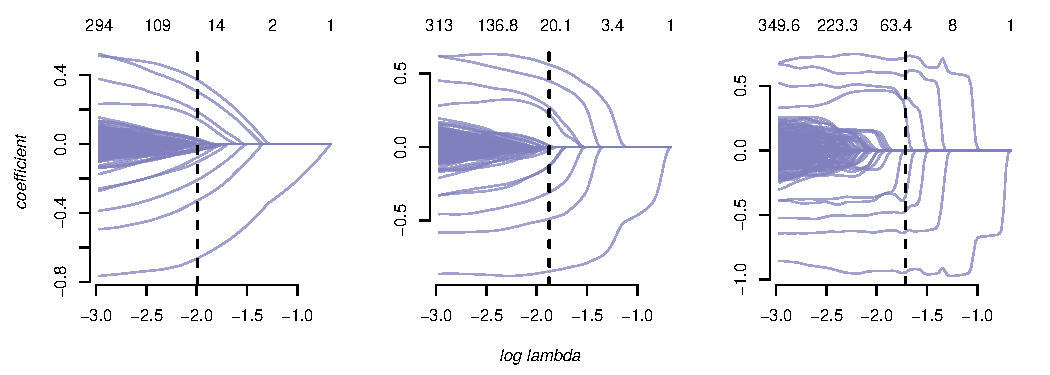
\includegraphics[width=6in]{sim_paths}
\caption{\label{simpaths} Regularization paths for simulation example.
Degrees of freedom $df^t$ are along the top. }
\vskip .3cm
{\small \hskip 2.5cm$\bs{\gamma=0}$\hskip 4cm$\bs{\gamma=2}$\hskip 4cm$\bs{\gamma=10}$}

~~~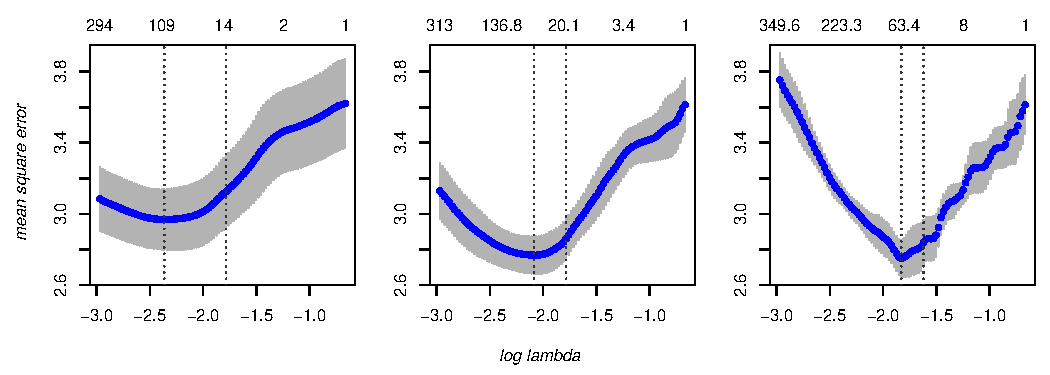
\includegraphics[width=6in]{sim_cv}
\caption{\label{simcv} 5-fold CV and AICc for a simulation example. 
Points-and-bars show mean OOS MSE $\pm 1$se.  }
\vspace{-.25cm}
\end{figure}

The regression in (\ref{simdgp}) is obviously {\it dense}:  true
coefficients are all nonzero.  However, they decay in magnitude along the
index $j$ and
it will be useless to estimate many of them in a $p=n$ regression.
Our sparse oracle comparator is the $C_p$ optimal $L_0$ penalized solution

\vspace{-.3cm}
\begin{equation}\label{l0oracle}
\bs{\beta}^{\star} = \argmin_{\bs{\beta}} \left\{ \|\bm{y}-\bm{X}\bs{\beta}\|^2 + 2\sigma^2\sum_j
\ds{1}_{\{\beta_j\neq0\}}\right\},
\end{equation} which is solvable here by searching through
OLS regression on $\bm{X}_{\{1\ldots j\}}$ for $j=1\ldots p$.

We consider {\tt gamlr} runs of GL with $\gamma$
of 0 (lasso), 2, and 10 and marginal AL, as well as
{\tt sparsenet}'s MCP penalized regression.  Covariate penalties are
standardized by $\mr{sd}(\bs{x}_j)$, and paths run through 100
$\lambda$ values down to $\lambda^{100} = 0.01\lambda^1$. On an Intel Xeon
E5-2670 core, 5-fold CV with $\mr{sd}(\bm{\eta})/\sigma=1$
and $\rho=1/2$ requires   1-2 seconds for lasso and marginal  AL, 2 and 3
seconds for GL with $\gamma=2$ and $\gamma=10$, and 15-20 seconds
for Sparsenet.
\footnote{{\tt ncvreg} SCAD required ten minutes for a single run and is thus
impractical for the applications under consideration.  But, in a small study,
CV.min selected SCAD performs quite well in prediction --  similarly to the
best CV.min methods for each data configuration -- with relatively high values
for both false discovery and sensitivity. }


Figures \ref{simpaths} and \ref{simcv} illustrate GL paths for a single
dataset, with  $\mr{sd}(\bm{\eta})/\sigma=1$ and $\rho=1/2$. In Figure
\ref{simpaths}, increasing $\gamma$ leads to `larger shouldered' paths where
estimates move quickly to MLE for the nonzero-coefficients. Degrees of
freedom, calculated as in (\ref{edf}), are along the top of each plot; equal
$\lambda$ have higher $df^t$ for higher $\gamma$ since there is less shrinkage
of $\hat\beta_j\neq0$.  Figure \ref{simcv} shows CV and AICc error estimates.
The two criteria roughly track each other, although AICc more heavily
penalizes over-fit and at $\gamma=10$ their minima do not match.  Notice that
as $\gamma$ increases, the CV error increases more quickly after it's minimum;
this indicates that the consequences of over-fit are worse under faster
diminishing bias.

% \begin{table}[p]\vspace{-.5cm}
% \caption[l]{\it Predictive Mean Square Error\hfill}
% \vspace{-.5cm}
% \small\setstretch{1}
% \begin{center}
% \begin{tabular}{l*{5}{c}|r}
%  & lasso & GL $\gamma=2$ & GL $\gamma=10$ & marginal AL & sparsenet MC+  &  \\
% \cline{1-7}
% CV.1se & 4.4 & 4.3 & 4.8 & 4.3 & 4.2 &\\
% CV.min & 4.1 & {\bf 4} & 4.3 & 4.1 & {\bf 4} &  $\mr{sd}(\bm{\mu})/\sigma=2$ \\
% AICc & 4.3 & 4.1 & 4.1 & 4.2 & & $\rho=0$ \\
% AIC & 5 & 5.2 & 5.2 & 4.1 & & \multirow{2}{*}{$C_p$ mse = 3.5} \\
% BIC & 5.6 & 5.1 & 5.7 & 4.9 & & \\
%  \hline 
% CV.1se & 3.1 & 3 & 3.4 & 3.1 & 2.9 &\\
% CV.min & 2.9 & {\bf 2.8} & 3 & 3 & {\bf 2.8} &  $\mr{sd}(\bm{\mu})/\sigma=2$ \\
% AICc & 3 & {\bf 2.8} & 2.9 & 3 & & $\rho=0.5$ \\
% AIC & 3.4 & 3.5 & 3.5 & 2.9 & & \multirow{2}{*}{$C_p$ mse = 2.4} \\
% BIC & 4.4 & 3.7 & 4.1 & 3.8 & & \\
%  \hline 
% CV.1se & 2.4 & 2.4 & 2.6 & 2.6 & 2.3 &\\
% CV.min & 2.3 & {\bf 2.2} & 2.3 & 2.4 & {\bf 2.2} &  $\mr{sd}(\bm{\mu})/\sigma=2$ \\
% AICc & 2.4 & {\bf 2.2} & 2.3 & 2.5 & & $\rho=0.9$ \\
% AIC & 2.6 & 2.7 & 2.7 & 2.4 & & \multirow{2}{*}{$C_p$ mse = 1.9} \\
% BIC & 3.5 & 3 & 3.3 & 3.2 & & \\
%  \hline 
% CV.1se & 17 & 16.9 & 18 & 15.6 & 16.4 &\\
% CV.min & 15.6 & 15.6 & 16.5 & 15.7 & 15.6 &  $\mr{sd}(\bm{\mu})/\sigma=1$ \\
% AICc & 15.8 & {\bf 15.5} & 15.9 & 15.6 & & $\rho=0$ \\
% AIC & 21.3 & 22.2 & 22.2 & 17 & & \multirow{2}{*}{$C_p$ mse = 13.8} \\
% BIC & 20.8 & 19.2 & 23.4 & 17.7 & & \\
%  \hline 
% CV.1se & 12 & 11.7 & 12.7 & 11.1 & 11.3 &\\
% CV.min & 10.9 & 10.8 & 11.5 & 11 & 10.8 &  $\mr{sd}(\bm{\mu})/\sigma=1$ \\
% AICc & 11.1 & {\bf 10.7} & 10.8 & 11 & & $\rho=0.5$ \\
% AIC & 14.4 & 14.9 & 14.9 & 11.8 & & \multirow{2}{*}{$C_p$ mse = 9.2} \\
% BIC & 15.8 & 14.4 & 16.1 & 13.4 & & \\
%  \hline 
% CV.1se & 9.4 & 9.2 & 10.1 & 9.1 & 8.9 &\\
% CV.min & 8.6 & {\bf 8.5} & 9 & 8.8 & {\bf 8.5} &  $\mr{sd}(\bm{\mu})/\sigma=1$ \\
% AICc & 8.8 & {\bf 8.5} & {\bf 8.5} & 8.8 & & $\rho=0.9$ \\
% AIC & 11.2 & 11.6 & 11.6 & 9.1 & & \multirow{2}{*}{$C_p$ mse = 7.3} \\
% BIC & 12.7 & 12.1 & 12.9 & 11.4 & & \\
%  \hline 
% CV.1se & 60.9 & 61.2 & 61.3 & 57.8 & 61 &\\
% CV.min & 57.8 & 59.8 & 60.6 & 60.5 & 57.9 &  $\mr{sd}(\bm{\mu})/\sigma=0.5$ \\
% AICc & {\bf 57.6} & 60 & 61.4 & 59 & & $\rho=0$ \\
% AIC & 88.4 & 92.5 & 92.5 & 73.2 & & \multirow{2}{*}{$C_p$ mse = 53.5} \\
% BIC & 61.3 & 61.3 & 61.3 & 60.6 & & \\
%  \hline 
% CV.1se & 41.1 & 41.2 & 41.2 & 39.8 & 41.2 &\\
% CV.min & 39.9 & 40.7 & 41 & 41.3 & 39.9 &  $\mr{sd}(\bm{\mu})/\sigma=0.5$ \\
% AICc & {\bf 39.6} & 40.5 & 41.3 & 40.5 & & $\rho=0.5$ \\
% AIC & 59.4 & 61.9 & 61.9 & 49.9 & & \multirow{2}{*}{$C_p$ mse = 35.9} \\
% BIC & 41.2 & 41.2 & 41.2 & 41 & & \\
%  \hline 
% CV.1se & 32.6 & 32.6 & 32.6 & 31.8 & 32.6 &\\
% CV.min & 31.8 & 32.3 & 32.5 & 32.4 & 31.8 &  $\mr{sd}(\bm{\mu})/\sigma=0.5$ \\
% AICc & {\bf 31.5} & 32.1 & 32.6 & 32.2 & & $\rho=0.9$ \\
% AIC & 46.4 & 48.6 & 48.6 & 38.1 & & \multirow{2}{*}{$C_p$ mse = 28.3} \\
% BIC & 32.6 & 32.6 & 32.6 & 32.5 & & \\
%  \hline \end{tabular}
% \end{center}
% \vspace{-1cm}
% \end{table}

\begin{table}[p]\vspace{-.5cm}
\caption[l]{\label{r2}\it Predictive $R^2$\hfill}
\vspace{-.5cm}
\small\setstretch{1}
\begin{center}
\begin{tabular}{l*{5}{c}|r}
 & lasso & GL $\gamma=2$ & GL $\gamma=10$ & marginal AL & sparsenet MCP  &  \\
\cline{1-7}
CV.1se & 0.71 & 0.72 & 0.68 & 0.72 & 0.73 &\\
CV.min & 0.73 & {\bf 0.74} & 0.72 & 0.73 & {\bf 0.74} &  $\mr{sd}(\bm{\mu})/\sigma=2$ \\
AICc & 0.72 & 0.73 & 0.73 & 0.73 & & $\rho=0$ \\
AIC & 0.67 & 0.66 & 0.66 & 0.73 & & \multirow{2}{*}{$C_p ~ R^2$ = 0.77} \\
BIC & 0.63 & 0.67 & 0.63 & 0.68 & & \\
 \hline 
CV.1se & 0.7 & 0.71 & 0.67 & 0.7 & 0.72 &\\
CV.min & 0.72 & {\bf 0.73} & 0.7 & 0.71 & {\bf 0.73} &  $\mr{sd}(\bm{\mu})/\sigma=2$ \\
AICc & 0.71 & {\bf 0.73} & 0.72 & 0.71 & & $\rho=0.5$ \\
AIC & 0.67 & 0.66 & 0.66 & 0.71 & & \multirow{2}{*}{$C_p ~ R^2$ = 0.77} \\
BIC & 0.57 & 0.64 & 0.6 & 0.63 & & \\
 \hline 
CV.1se & 0.7 & 0.71 & 0.68 & 0.68 & 0.72 &\\
CV.min & 0.72 & {\bf 0.73} & 0.71 & 0.7 & {\bf 0.73} &  $\mr{sd}(\bm{\mu})/\sigma=2$ \\
AICc & 0.71 & {\bf 0.73} & 0.72 & 0.7 & & $\rho=0.9$ \\
AIC & 0.68 & 0.67 & 0.67 & 0.7 & & \multirow{2}{*}{$C_p ~ R^2$ = 0.77} \\
BIC & 0.57 & 0.63 & 0.6 & 0.61 & & \\
 \hline 
CV.1se & 0.31 & 0.31 & 0.27 & 0.36 & 0.33 &\\
CV.min & 0.36 & 0.36 & 0.33 & 0.36 & 0.36 &  $\mr{sd}(\bm{\mu})/\sigma=1$ \\
AICc & 0.35 & {\bf 0.37} & 0.35 & 0.36 & & $\rho=0$ \\
AIC & 0.13 & 0.09 & 0.09 & 0.3 & & \multirow{2}{*}{$C_p ~ R^2$ = 0.44} \\
BIC & 0.15 & 0.22 & 0.04 & 0.28 & & \\
 \hline 
CV.1se & 0.27 & 0.29 & 0.23 & 0.33 & 0.32 &\\
CV.min & 0.34 & {\bf 0.35} & 0.3 & 0.33 & {\bf 0.35} &  $\mr{sd}(\bm{\mu})/\sigma=1$ \\
AICc & 0.32 & {\bf 0.35} & {\bf 0.35} & 0.33 & & $\rho=0.5$ \\
AIC & 0.12 & 0.1 & 0.1 & 0.28 & & \multirow{2}{*}{$C_p ~ R^2$ = 0.44} \\
BIC & 0.04 & 0.13 & 0.02 & 0.19 & & \\
 \hline 
CV.1se & 0.28 & 0.29 & 0.23 & 0.3 & 0.31 &\\
CV.min & 0.34 & {\bf 0.35} & 0.31 & 0.32 & {\bf 0.35} &  $\mr{sd}(\bm{\mu})/\sigma=1$ \\
AICc & 0.33 & {\bf 0.35} & {\bf 0.35} & 0.32 & & $\rho=0.9$ \\
AIC & 0.14 & 0.11 & 0.11 & 0.3 & & \multirow{2}{*}{$C_p ~ R^2$ = 0.44} \\
BIC & 0.03 & 0.07 & 0.01 & 0.13 & & \\
 \hline 
CV.1se & 0.01 & 0 & 0 & {\bf 0.06} & 0 &\\
CV.min & {\bf 0.06} & 0.02 & 0.01 & 0.01 & 0.05 &  $\mr{sd}(\bm{\mu})/\sigma=0.5$ \\
AICc & {\bf 0.06} & 0.02 & 0 & 0.04 & & $\rho=0$ \\
AIC & -0.44 & -0.51 & -0.51 & -0.2 & & \multirow{2}{*}{$C_p ~ R^2$ = 0.13} \\
BIC & 0 & 0 & 0 & 0.01 & & \\
 \hline 
CV.1se & 0 & 0 & 0 & 0.03 & 0 &\\
CV.min & 0.03 & 0.01 & 0 & -0.01 & 0.03 &  $\mr{sd}(\bm{\mu})/\sigma=0.5$ \\
AICc & {\bf 0.04} & 0.01 & 0 & 0.01 & & $\rho=0.5$ \\
AIC & -0.45 & -0.51 & -0.51 & -0.21 & & \multirow{2}{*}{$C_p ~ R^2$ = 0.13} \\
BIC & 0 & 0 & 0 & 0 & & \\
 \hline 
CV.1se & 0 & 0 & 0 & 0.02 & 0 &\\
CV.min & 0.02 & 0.01 & 0 & 0 & 0.02 &  $\mr{sd}(\bm{\mu})/\sigma=0.5$ \\
AICc & {\bf 0.03} & 0.01 & 0 & 0.01 & & $\rho=0.9$ \\
AIC & -0.43 & -0.5 & -0.5 & -0.17 & & \multirow{2}{*}{$C_p ~ R^2$ = 0.13} \\
BIC & 0 & 0 & 0 & 0 & & \\
 \hline 
\end{tabular}
\end{center}
\vspace{-1cm}
\end{table}

\begin{table}[p]\vspace{-.5cm}
\caption[l]{\label{sens}\it False Discovery Rate $\mid$ Sensitivity, relative to $C_p$ model\hfill}
\vspace{-.5cm}
\small\setstretch{1}
\begin{center}
\begin{tabular}{l*{5}{c}|r}
 & lasso & GL $\gamma=2$ & GL $\gamma=10$ & marginal AL & sparsenet MCP  & \\
 \cline{1-7}
CV.1se & 0.49 $\mid$ 0.76 & 0.26 $\mid$ 0.67 & 0.07 $\mid$ 0.56 & 0.43 $\mid$ 0.67 & 0.15 $\mid$ 0.61 &\\
CV.min & 0.65 $\mid$ 0.84 & 0.48 $\mid$ 0.77 & 0.20 $\mid$ 0.65 & 0.57 $\mid$ 0.74 & 0.40 $\mid$ 0.74 &  $\mr{sd}(\bm{\mu})/\sigma=2$ \\
AICc & 0.55 $\mid$ 0.79 & 0.44 $\mid$ 0.76 & 0.37 $\mid$ 0.73 & 0.53 $\mid$ 0.71 & & $\rho=0$ \\
AIC & 0.84 $\mid$ 0.94 & 0.84 $\mid$ 0.93 & 0.84 $\mid$ 0.91 & 0.63 $\mid$ 0.77 & & \multirow{2}{*}{$\bar{s}_{C_p}$ = 123.7} \\
BIC & 0.22 $\mid$ 0.59 & 0.07 $\mid$ 0.53 & 0.02 $\mid$ 0.45 & 0.22 $\mid$ 0.54 & & \\
 \hline 
CV.1se & 0.58 $\mid$ 0.75 & 0.37 $\mid$ 0.67 & 0.12 $\mid$ 0.55 & 0.53 $\mid$ 0.64 & 0.14 $\mid$ 0.58 &\\
CV.min & 0.69 $\mid$ 0.84 & 0.56 $\mid$ 0.77 & 0.27 $\mid$ 0.65 & 0.63 $\mid$ 0.71 & 0.34 $\mid$ 0.69 &  $\mr{sd}(\bm{\mu})/\sigma=2$ \\
AICc & 0.60 $\mid$ 0.77 & 0.50 $\mid$ 0.74 & 0.41 $\mid$ 0.73 & 0.59 $\mid$ 0.69 & & $\rho=0.5$ \\
AIC & 0.84 $\mid$ 0.94 & 0.84 $\mid$ 0.94 & 0.84 $\mid$ 0.92 & 0.67 $\mid$ 0.75 & & \multirow{2}{*}{$\bar{s}_{C_p}$ = 123.5} \\
BIC & 0.29 $\mid$ 0.53 & 0.13 $\mid$ 0.49 & 0.04 $\mid$ 0.44 & 0.31 $\mid$ 0.49 & & \\
 \hline 
CV.1se & 0.59 $\mid$ 0.76 & 0.43 $\mid$ 0.67 & 0.21 $\mid$ 0.56 & 0.54 $\mid$ 0.61 & 0.20 $\mid$ 0.57 &\\
CV.min & 0.69 $\mid$ 0.84 & 0.57 $\mid$ 0.77 & 0.35 $\mid$ 0.66 & 0.63 $\mid$ 0.69 & 0.41 $\mid$ 0.69 &  $\mr{sd}(\bm{\mu})/\sigma=2$ \\
AICc & 0.61 $\mid$ 0.77 & 0.52 $\mid$ 0.74 & 0.43 $\mid$ 0.71 & 0.60 $\mid$ 0.66 & & $\rho=0.9$ \\
AIC & 0.84 $\mid$ 0.94 & 0.84 $\mid$ 0.93 & 0.83 $\mid$ 0.91 & 0.65 $\mid$ 0.71 & & \multirow{2}{*}{$\bar{s}_{C_p}$ = 123.9} \\
BIC & 0.35 $\mid$ 0.51 & 0.20 $\mid$ 0.47 & 0.09 $\mid$ 0.43 & 0.39 $\mid$ 0.47 & & \\
 \hline 
CV.1se & 0.43 $\mid$ 0.58 & 0.18 $\mid$ 0.44 & 0.07 $\mid$ 0.33 & 0.52 $\mid$ 0.62 & 0.26 $\mid$ 0.50 &\\
CV.min & 0.66 $\mid$ 0.73 & 0.43 $\mid$ 0.60 & 0.19 $\mid$ 0.45 & 0.68 $\mid$ 0.73 & 0.57 $\mid$ 0.69 &  $\mr{sd}(\bm{\mu})/\sigma=1$ \\
AICc & 0.60 $\mid$ 0.69 & 0.50 $\mid$ 0.65 & 0.50 $\mid$ 0.63 & 0.62 $\mid$ 0.69 & & $\rho=0$ \\
AIC & 0.90 $\mid$ 0.93 & 0.90 $\mid$ 0.92 & 0.90 $\mid$ 0.89 & 0.79 $\mid$ 0.82 & & \multirow{2}{*}{$\bar{s}_{C_p}$ = 90.0} \\
BIC & 0.07 $\mid$ 0.25 & 0.04 $\mid$ 0.25 & 0.00 $\mid$ 0.04 & 0.17 $\mid$ 0.38 & & \\
 \hline 
CV.1se & 0.52 $\mid$ 0.54 & 0.30 $\mid$ 0.43 & 0.12 $\mid$ 0.32 & 0.61 $\mid$ 0.58 & 0.23 $\mid$ 0.42 &\\
CV.min & 0.70 $\mid$ 0.71 & 0.53 $\mid$ 0.60 & 0.27 $\mid$ 0.45 & 0.71 $\mid$ 0.69 & 0.47 $\mid$ 0.58 &  $\mr{sd}(\bm{\mu})/\sigma=1$ \\
AICc & 0.65 $\mid$ 0.66 & 0.56 $\mid$ 0.63 & 0.56 $\mid$ 0.65 & 0.67 $\mid$ 0.65 & & $\rho=0.5$ \\
AIC & 0.90 $\mid$ 0.94 & 0.90 $\mid$ 0.93 & 0.90 $\mid$ 0.91 & 0.81 $\mid$ 0.81 & & \multirow{2}{*}{$\bar{s}_{C_p}$ = 90.0} \\
BIC & 0.03 $\mid$ 0.07 & 0.05 $\mid$ 0.15 & 0.00 $\mid$ 0.03 & 0.21 $\mid$ 0.26 & & \\
 \hline 
CV.1se & 0.57 $\mid$ 0.54 & 0.40 $\mid$ 0.43 & 0.23 $\mid$ 0.30 & 0.62 $\mid$ 0.53 & 0.32 $\mid$ 0.40 &\\
CV.min & 0.71 $\mid$ 0.72 & 0.57 $\mid$ 0.60 & 0.38 $\mid$ 0.45 & 0.70 $\mid$ 0.65 & 0.55 $\mid$ 0.58 &  $\mr{sd}(\bm{\mu})/\sigma=1$ \\
AICc & 0.66 $\mid$ 0.66 & 0.58 $\mid$ 0.61 & 0.58 $\mid$ 0.62 & 0.69 $\mid$ 0.62 & & $\rho=0.9$ \\
AIC & 0.90 $\mid$ 0.94 & 0.90 $\mid$ 0.92 & 0.90 $\mid$ 0.90 & 0.80 $\mid$ 0.77 & & \multirow{2}{*}{$\bar{s}_{C_p}$ = 89.7} \\
BIC & 0.03 $\mid$ 0.04 & 0.05 $\mid$ 0.08 & 0.00 $\mid$ 0.01 & 0.21 $\mid$ 0.17 & & \\
 \hline 
CV.1se & 0.07 $\mid$ 0.05 & 0.01 $\mid$ 0.01 & 0.01 $\mid$ 0.01 & 0.65 $\mid$ 0.45 & 0.07 $\mid$ 0.04 &\\
CV.min & 0.61 $\mid$ 0.41 & 0.20 $\mid$ 0.13 & 0.07 $\mid$ 0.05 & 0.80 $\mid$ 0.63 & 0.59 $\mid$ 0.40 &  $\mr{sd}(\bm{\mu})/\sigma=0.5$ \\
AICc & 0.64 $\mid$ 0.43 & 0.49 $\mid$ 0.34 & 0.02 $\mid$ 0.01 & 0.76 $\mid$ 0.57 & & $\rho=0$ \\
AIC & 0.94 $\mid$ 0.92 & 0.94 $\mid$ 0.90 & 0.94 $\mid$ 0.90 & 0.90 $\mid$ 0.81 & & \multirow{2}{*}{$\bar{s}_{C_p}$ = 56.5} \\
BIC & 0.00 $\mid$ 0.01 & 0.00 $\mid$ 0.00 & 0.00 $\mid$ 0.00 & 0.07 $\mid$ 0.05 & & \\
 \hline 
CV.1se & 0.04 $\mid$ 0.01 & 0.01 $\mid$ 0.00 & 0.00 $\mid$ 0.00 & 0.70 $\mid$ 0.35 & 0.09 $\mid$ 0.01 &\\
CV.min & 0.56 $\mid$ 0.25 & 0.20 $\mid$ 0.07 & 0.08 $\mid$ 0.03 & 0.82 $\mid$ 0.56 & 0.54 $\mid$ 0.24 &  $\mr{sd}(\bm{\mu})/\sigma=0.5$ \\
AICc & 0.65 $\mid$ 0.31 & 0.43 $\mid$ 0.26 & 0.05 $\mid$ 0.03 & 0.79 $\mid$ 0.49 & & $\rho=0.5$ \\
AIC & 0.94 $\mid$ 0.93 & 0.94 $\mid$ 0.91 & 0.94 $\mid$ 0.91 & 0.91 $\mid$ 0.80 & & \multirow{2}{*}{$\bar{s}_{C_p}$ = 56.3} \\
BIC & 0.01 $\mid$ 0.00 & 0.00 $\mid$ 0.00 & 0.00 $\mid$ 0.00 & 0.06 $\mid$ 0.02 & & \\
 \hline 
CV.1se & 0.03 $\mid$ 0.01 & 0.01 $\mid$ 0.00 & 0.00 $\mid$ 0.00 & 0.68 $\mid$ 0.25 & 0.14 $\mid$ 0.01 &\\
CV.min & 0.53 $\mid$ 0.19 & 0.23 $\mid$ 0.05 & 0.08 $\mid$ 0.02 & 0.82 $\mid$ 0.49 & 0.52 $\mid$ 0.17 &  $\mr{sd}(\bm{\mu})/\sigma=0.5$ \\
AICc & 0.67 $\mid$ 0.27 & 0.41 $\mid$ 0.21 & 0.04 $\mid$ 0.03 & 0.80 $\mid$ 0.44 & & $\rho=0.9$ \\
AIC & 0.94 $\mid$ 0.93 & 0.94 $\mid$ 0.90 & 0.94 $\mid$ 0.90 & 0.90 $\mid$ 0.76 & & \multirow{2}{*}{$\bar{s}_{C_p}$ = 55.8} \\
BIC & 0.01 $\mid$ 0.00 & 0.00 $\mid$ 0.00 & 0.00 $\mid$ 0.00 & 0.08 $\mid$ 0.01 & & \\
 \hline 
 \end{tabular}
\end{center}
\vspace{-1cm}
\end{table}


Results over a set of 1000 datasets are presented in Tables \ref{r2} and
\ref{sens}.  The first table records out-of-sample $R^2 = 1 -
\mr{var}(\bm{\tilde y} - \bs{\eta}_\bm{y})/\mr{var}(\bm{\tilde y})$, while the
second reports false discovery and sensitivity with respect to the $L_0$
oracle of (\ref{l0oracle}).  For $\mr{sd}(\bm{\eta})/\sigma$ of $1$ to $2$,
the highest $R^2$ values are obtained by CV.min  MCP and  by $\gamma=2$  GL
with either CV.min or AICc selection. When $\mr{sd}(\bm{\eta})/\sigma$ drops
to $1/2$, the top performer is AICc lasso. Investigation of the AICc values
finds that $\gamma=0$ was consistently favored over $\gamma=2$ in this low
signal setting, so that AICc selection on just two GL paths (for each of
$\gamma=0$ and $1$) would have been enough to get the best predictor in all
scenarios.\footnote{Note also the massive improvement of AICc over AIC: the
latter leads to negative $R^2$.} No algorithm ever does more than 1-2\% better
than lasso, but the sparser (e.g., $\gamma=10$) fits do nearly as
well as best in all but the low signal settings, where all but lasso suffer.

In Table \ref{sens}, where the false
discovery rate (FDR) $\sum_j\ds{1}_{\{\hat\beta_j \neq 0 \cap
\beta^\star_j=0\}}/\sum_j\ds{1}_{\{\hat\beta_j \neq 0\}}$ needs to be balanced
against sensitivity $\sum_j\ds{1}_{\{\hat\beta_j \neq 0 \cap \beta^\star_j
\neq 0\}}/\sum_j\ds{1}_{\{\beta^\star_j \neq 0\}}$, results are less
straightforward.  If false discovery is the primary concern, then you do well
using GL with $\gamma=10$; for example, under CV.1se selection when
$\mr{sd}(\bm{\eta})/\sigma=1$ and $\rho=1/2$, $\gamma=10$ GL has FDR of 0.12
against lasso's 0.52 and MCP's 0.23.  But this does come at the expense of a
drop in sensitivity, to 0.32 from lasso's 0.54 and MCP's 0.42. Across all
routines,  CV.1se selection  appears to do the best job of controlling
FDR without too dramatically under-fitting.  In any case, it appears that you
should use small $\gamma$ when focused on prediction and large $\gamma$ when
FDR is a primary concern.


\section{Hockey players}
\label{nhl}


This section attempts to quantify the
performance of hockey players.  It extends  analysis in
\cite{gramacy_estimating_2013}.  The current version includes data about who
was on the ice for every goal in the National Hockey League (NHL) back to the
2002-2003 season, including playoffs.  The data
are in the {\tt gamlr} package; there are
69449 goals and 2439 players.


The logistic regression model of player contribution is, for goal $i$ in
season $s$ with away team $a$ and home team $h$,
\begin{align}\label{hockeymod}
\mr{logit}\left[\mr{p}(\text{home~team~scored~goal}~i)\right] = \alpha_0 +
\alpha_{sh} - \alpha_{sa} + \bm{u}_i'\bs{\phi} + \bm{x}_i'\bs{\beta}_0 +
\bm{x}_i'\bs{\beta}_s, \end{align}  Vector $\bm{u}_i$ holds indicators for
various special-teams scenarios (e.g., a home team power play), and
$\bs{\alpha}$ provides matchup/season specific intercepts. Vector $\bm{x}_i$
contains player effects: $x_{ij}=1$ if player $j$ was on the home team and on
ice for goal $i$, $x_{ij}=-1$ for away player $j$ on ice for goal $i$, and
$x_{ij}=0$ for everyone not on the ice.   Coefficient $\beta_{0j} +
\beta_{sj}$ is the season-$s$ effect of player $j$ on the log odds that, given
a goal has been scored, the goal was scored by their team.  These effects are
`partial' in that they control for who else was on the ice, special teams
scenarios, and team-season fixed effects -- a player's $\beta_{0j}$ or $\beta_{sj}$
only need be nonzero if that player effects play above or below the team
average for a given season.

We estimate gamma lasso paths of $\bs{\beta}$ for the model in
(\ref{hockeymod}) {\it with  $\bs{\alpha}$ and $\bs{\phi}$ left unpenalized}.
In contrast to the default for most analyses, our coefficient costs are {\it
not} scaled by covariate standard deviation.  Doing the usual standardization
would have favored players with little ice time.  The algorithm is run for
$\log_{10}\gamma = -5 \ldots 2$, plus the $\gamma=0$ lasso.\footnote{On this
data, $\gamma=\infty$ subset selection yields perfect separation and infinite
likelihood.}

Joint $[\gamma,\lambda]$ surfaces for AICc and BIC are in Figure \ref{nhlic}.
AICc favors denser models with low $\lambda$ but not-to-big $\gamma$,
while the BIC  prefers very sparse but relatively unbiased  models with large
$\lambda$ and small $\gamma$.  Both criteria are strongly adverse to any model
at $\gamma=100$, which is where timings explode in Figure
\ref{nhltime}.  Ten-fold CV results are shown in Figure
\ref{nhlcv} for $\gamma$ of 0, 1, and 10.  The OOS error minima are around the
same in each case -- average deviance slightly above 1.16 -- but errors
increase much faster away from optimality with larger $\gamma$.   We also see
that AICc selection is always between the CV.min and CV.1se selctions:  at
$\gamma=0$ AICc matches the CV.1se choice, while at $\gamma=10$ it has moved
right to the CV.1se  selection.  Our heuristic from Section \ref{dof} might be
over-estimating $df$ for large-$\gamma$ models (especially under this very
collinear design), but one would also suspect that CV estimates of minimum
deviance are biased downward more dramatically for larger $\gamma$ than for
low-variance small-$\gamma$ estimators.



\begin{figure}[tb]
\begin{center}\vskip -.5cm
~~~~~~~~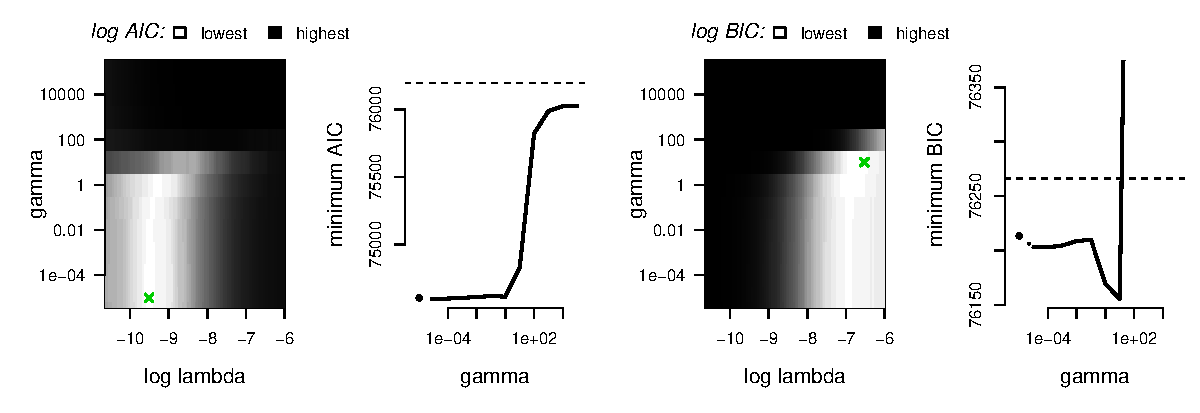
\includegraphics[width=5in]{nhl_ic}
\caption{ \label{nhlic} Hockey example AICc and BIC surfaces, rising from white to black on log scale.
}
\end{center}
% \end{figure}
% \begin{figure}[htb]
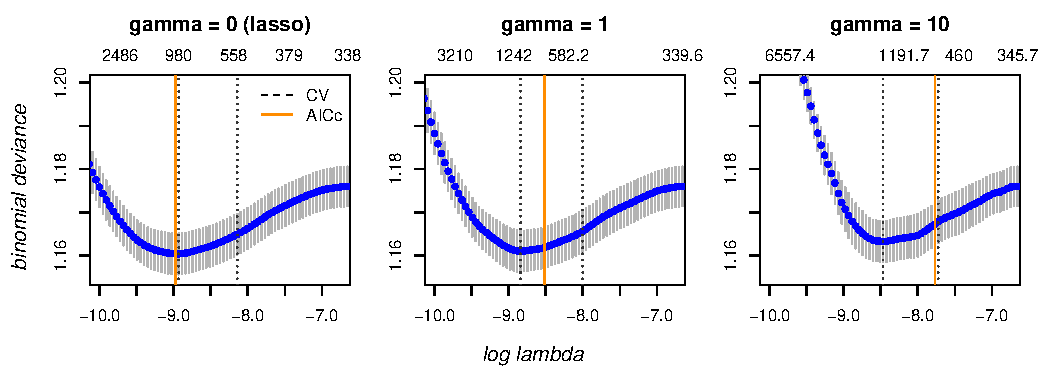
\includegraphics[width=6.3in]{nhl_cv}
\caption{\label{nhlcv} Hockey example 10-fold CV: mean OOS deviance $\pm 1$se, with minimum-error and 1SE selection rules marked with black dotted lines, and solid orange line showing AICc selection. }
\end{figure}


\begin{table}[tb]\footnotesize\setstretch{1}
\makebox[\linewidth]{
\begin{tabular}{l|lcc|lcc|lcc|}
\multicolumn{1}{c}{} & \multicolumn{3}{l}{\normalsize \it ~~~lasso} & \multicolumn{3}{l}{\normalsize \it ~~~$\gamma=1$} &  \multicolumn{3}{l}{\normalsize \it ~~~$\gamma=10$}\\
%\multicolumn{1}{c}{} & \multicolumn{3}{r|}{} & \multicolumn{3}{r|}{} &  \multicolumn{3}{r|}{}\\
\multicolumn{1}{c}{}  &     &    PPM & PM &    &   PPM & PM        &   & PPM & PM \\
\cline{3-4}\cline{6-7}\cline{9-10}
1 & Ondrej Palat & 33.8 & 14 & Sidney Crosby & 29.2 & -4 & Sidney Crosby & 32.6 & -4 \\
2 & Sidney Crosby & 31.2 & -4 & Ondrej Palat & 29 & 14 & Jonathan Toews & 22.8 & 5 \\
3 & Henrik Lundqvist & 25.8 & 49 & Jonathan Toews & 21.4 & 5 & Joe Thornton & 22 & -22 \\
4 & Jonathan Toews & 24 & 5 & Joe Thornton & 21 & -22 & Anze Kopitar & 22 & 29 \\
5 & Andrei Markov & 23.1 & -6 & Andrei Markov & 20.9 & -6 & Andrei Markov & 20.7 & -6 \\
6 & Joe Thornton & 21.4 & -22 & Henrik Lundqvist & 19.8 & 49 & Alex Ovechkin & 18.1 & -14 \\
7 & Anze Kopitar & 20.6 & 29 & Anze Kopitar & 19.5 & 29 & Pavel Datsyuk & 16.6 & -13 \\
8 & Tyler Toffoli & 18.9 & 11 & Pavel Datsyuk & 16.1 & -13 & Ryan Getzlaf & 15.8 & -34 \\
9 & Pavel Datsyuk & 17.7 & -13 & Logan Couture & 15.9 & -27 & Henrik Sedin & 15.2 & -9 \\
10 & Ryan Nugent & 17.4 & 2 & Alex Ovechkin & 15.8 & -14 & Marian Hossa & 14.9 & 3 \\
11 & Gabriel Landeskog & 16.6 & 26 & Marian Hossa & 14.4 & 3 & Alexander Semin & 14.7 & 17 \\
12 & Logan Couture & 16.5 & -27 & Alexander Semin & 14.2 & 17 & Jaromir Jagr & 14.5 & 2 \\
13 & Alex Ovechkin & 15.8 & -14 & Matt Moulson & 13.9 & 12 & Logan Couture & 14.2 & -27 \\
14 & Marian Hossa & 15.4 & 3 & Tyler Toffoli & 13.3 & 11 & Matt Moulson & 13.7 & 12 \\
15 & Alexander Semin & 14.8 & 17 & David Perron & 12.7 & 2 & Mikko Koivu & 13 & -4 \\
16 & Zach Parise & 14.7 & -9 & Mikko Koivu & 12.5 & -4 & Joe Pavelski & 12.6 & -15 \\
17 & Frans Nielsen & 13.5 & -16 & Frans Nielsen & 12.3 & -16 & Steven Stamkos & 12.6 & 24 \\
18 & Mikko Koivu & 13.4 & -4 & Ryan Getzlaf & 12.1 & -34 & Frans Nielsen & 12.5 & -16 \\
19 & Matt Moulson & 13.4 & 12 & Ryan Nugent & 11.9 & 2 & Marian Gaborik & 12.3 & 5 \\
20 & David Perron & 13.1 & 2 & Jaromir Jagr & 11.8 & 2 & Zach Parise & 12.2 & -9 \\
% 21 & Joe Pavelski & 12.4 & -15 & Joe Pavelski & 11.5 & -15 & Tobias Enstrom & 10.9 & 21 \\
% 22 & Jordan Eberle & 12.4 & 9 & Marian Gaborik & 11.4 & 5 & Daniel Alfredsson & 10.7 & -9 \\
% 23 & Radim Vrbata & 12.3 & 16 & Zach Parise & 11.2 & -9 & Radim Vrbata & 10.1 & 16 \\
% 24 & Jakub Voracek & 12.3 & 12 & Jordan Eberle & 10.8 & 9 & Rick Nash & 9.9 & 16 \\
% 25 & Marian Gaborik & 12.1 & 5 & Radim Vrbata & 10.5 & 16 & Vincent Lecavalier & 9.4 & 9 \\
\multicolumn{1}{c}{} & \multicolumn{3}{r|}{} & \multicolumn{3}{r|}{} &  \multicolumn{3}{r|}{}\\
 \multicolumn{1}{c}{} & \multicolumn{3}{r|}{\it 305 nonzero effects} & \multicolumn{3}{r|}{\it 204 nonzero effects} &  \multicolumn{3}{r|}{\it 64 nonzero effects}
\end{tabular}}
\caption{\label{nhleffects} Top 20 AICc selected player `partial plus-minus' (PPM) values for the 2013-2014 season, under $\gamma = 0,1,10$.  The number of nonzero player effects for each $\gamma$ are noted along the bottom.}
\end{table}

The motivating application for this example was to devise a better versions of
hockey's `plus-minus' (PM) statistic: number of goals {\it for} minus {\it
against} each player's team while he is on the ice. To convert from player
effects $\beta_{0j} + \beta_{sj}$ to the scale of `plus/minus', we first state
that in absence of any other relevant information about each goal (not team,
home/away, etc), the probability a goal was scored by his team given player
$j$ is on ice becomes $p_j = e^{\beta_j}/(1+e^{\beta_j})$ and our `partial
plus/minus' (PPM) is \[ \mr{ppm}_j = N_j(p_j - (1-p_j)) = N_j(2p_j-1) \] where
$N_j$ is the  number of goals for which he was on-ice.  This measures 
quality and quantity of contribution, controlling for
confounding information, and lives on the same scale as PM.

Table \ref{nhleffects} contains the estimated PPM values for the 2013-2014
season under various $\gamma$ levels, using AICc selection.  We see that, even
if changing concavity ($\gamma$) has little effect on minimum CV errors,
larger $\gamma$  yield more sparse models and different conclusions about
player contribution. At the $\gamma=0$ lasso, there are 305 nonzero player
effects (individuals measurably different from their team's average ability)
and the list includes young players who have had very strong starts to their
careers.  For example, Ondrej Palat and Tyler Toffoli both played their first
full seasons in the NHL in 2013-2014.  As $\gamma$ increases to 1, these young
guys  drop in rank while more proven stars (e.g., Sidney Crosby and Jonathan
Toews) move up the list.  Finally, at $\gamma=10$ only big-name stars remain
amongst the 64 nonzero player effects.

\section{Discussion}
\label{discussion}

Diminishing bias estimation in Big data, where exact solvers are too
computationally expensive, reduces largely to weighted $L_1$ penalization.
This review has covered a number of topics that we think relevant for such
schemes: theoretical distance to $L_0$ minimization, relationship to a
Bayesian model, and stability, degrees of freedom, and estimates of predictive
performance along entire regularization paths. We have described a world where
model selection is considered throughout construction of candidate models, not
as an afterthought, and where one seeks sparse representations even for
non-sparse truth.
 
Apart from the simulation study, we have not provided extensive comparison of
the many available weighting mechanisms. Our gamma lasso performs as well as
or better than adaptive lasso and MCP penalized alternatives in simulation,
but we are not arguing that its path-based weights are theoretically optimal.
For example, instead of moving {\it forward} from higher to lower penalties,
\cite{van_de_geer_adaptive_2011} argue for a single {\it backward} step 
where the weights are based on initial coefficient values estimated under less
penalty than is used in the final fit.  The backwards approach will be more
expensive and the weights should have higher sampling variance, but we are
happy to believe that it can yield better support recovery properties.

The gamma lasso does have the advantage that using a regularization path to
supply penalty weights is computationally efficient. To scale for truly Big
data, $L_1$ weights need be constructed at practically no cost on top of a
standard lasso run. Beyond {\tt gamlr} and marginal regression adaptive lasso,
we have found no other software where this standard is met.


\appendix
\vskip 1cm
\noindent{\bf\Large Appendices}

\section{Gradient, curvature, and path starts}
\label{models}

The negative log likelihood objective in Gaussian regression is $
l(\alpha,\bs{\beta}) = 0.5\sum_i (y_i -\eta_i)^2 $ with gradient
$g_j(\bs{\beta}) = \partial l/\partial \beta_j = -\sum_i x_{ij}(y_i -
\eta_i)$, and coordinate curvature $h_j(\bs{\beta}) = \partial^2 l/\partial
\beta_j^2 = \sum_i x_{ij}^2$. In logistic regression, set $y_i = 1$ for
`success' and $y_i = 0$ for `failure' and write $q_i = (1 +
\exp[-\eta_i])^{-1}$ as the probability of success.  Then
$l(\alpha,\bs{\beta}) = \sum_i -y_i\eta_i + \log(1 +
  \exp[\eta_i])$,
$
g_j(\bs{\beta}) = \partial l/\partial \beta_j = -\sum_i
x_{ij}(y_i - q_i)$, and
$h_j(\bs{\beta}) = \partial^2 l/\partial \beta_j^2 = \sum_i
x_{ij}^2q_i(1-q_i)
$.
In each case, it is implied that $\hat\alpha$ has been set
to minimize $l(\alpha,\bs{\hat\beta})$. 

For $L_1$ costs $c_j(|\beta_j|) = |\beta_j|$, the infimum $\lambda$ such
that $\bs{\hat\beta} = \bm{0}$ is  available analytically as
$\lambda^1 =
n^{-1}\max\{|g_j(\bm{0})|,~j=1\ldots p\}$, the maximum mean
absolute gradient for the null model with $\bs{\beta} = \bm{0}$.  This formula
is used to obtain our starting values for the path algorithms.

\section{Implementation via coordinate descent}
\label{implement}

We use Coordinate descent \citep[CD; e.g.,][]{luenberger_linear_2008} to minimize
(\ref{l1pen}) at each step along the path. CD is a local optimization
algorithm that cycles through minimization of the conditional objective for
individual parameters when the remaining parameters are fixed. Algorithms of this type have have become popular in
$L_1$ penalized estimation since the work by \citet{friedman_pathwise_2007} and
\citet{wu_coordinate_2008}.

Our CD routine, outlined in Algorithm \ref{bmove}, is a solver for penalized
weighted least squares problems as defined in equation (\ref{newton}) below.
This applies directly in Gaussian regression, and for non-Gaussian models  we
follow \citet{friedman_regularization_2010} and apply CD inside an outer loop
of iteratively re-weighted least-squares \citep[IRLS;
e.g.,][]{green_iteratively_1984}. Given current parameter values
$\bs{\hat\beta}$, the Newton-Raphson update for maximum likelihood estimation
is $\bs{\beta} = \bs{\hat\beta} - \bm{H}^{-1}\bm{g}$, where $\bm{H}$ is the
information matrix with elements $h_{jk} = \partial^2 l/\partial
\beta_j\partial \beta_k |_{\bs{\hat\beta}}$ and $\bm{g}$ is coefficient
gradient (see Appendix \ref{models}). For exponential family linear models we
can write $\bm{H} = \bm{X}'\bm{V}\bm{X}$ and $\bm{g} = \bm{X}'\bm{V}(\bm{z} -
\bs{\hat\eta})$, where $\bm{V} = \mr{diag}(\bm{v})$, $\bm{v} = [v_1\ldots
v_n]$ are `weights', $\bm{z} = [z_1\ldots z_n]$ are transformed `response',
and $\hat\eta_i = \hat\alpha + \bm{x}_i\bs{\hat\beta}$.  In Gaussian
regression,  $v_i = 1$, $z_i=\hat\eta_i - y_i$, and the update is an exact
solution. For binomial regression, $v_i = q_i(1-q_i)$ and $z_i = \hat\eta_i -
(y_i-q_i)/v_i$, where $q_i = (1 + \exp[-\hat\eta_i])^{-1}$ is the  estimated
probability of success.

This yields $\bs{\beta} = (\bm{X}'\bm{V}\bm{X})^{-1}\bm{X}'\bm{V}\bm{z}$, such
that the Newton update solves a weighted least-squares problem.   Adding $L_1$
costs,  the minimization objective from (\ref{l1pen}) becomes
\begin{equation} \label{newton}  \argmin_{\alpha,\beta_1 \ldots \beta_p \in
\ds{R}} \sum_i \frac{v_i}{2}(\alpha + \bm{x}_i'\bs{\beta} - z_i)^2  + n\sum_j \omega_j
\lambda |\beta_j|. \end{equation} Our solver iterates between CD on
(\ref{newton}) and,  for non-Gaussian models, updates to $\bm{v}$ and
$\bm{z}$. Each $t^{th}$ segment IRLS routine initializes $[\hat \alpha,
\bs{\hat \beta}]$ at solutions for $\lambda^{t-1}$, or at $[\hat \alpha,
\bm{0}]$ for $t=1$.  In the {\tt gamlr} implementation, a full pass update of
all parameters is done only at the first CD iteration; otherwise coordinates
with currently inactive (zero) $\hat\beta_j$ are not updated. Once the descent
converges for this {\it active set}, IRLS $\bm{v}$ and $\bm{z}$ are updated
and we begin a new CD loop with a full pass update.  The routine stops when
maximum squared change in $\beta_j$ scaled by its information over one of
these full pass updates is less than some tolerance threshold, ${\tt thresh}$.
The default in {\tt gamlr} uses a relative tolerance of $10^{-7}$ times null
model deviance.  

\vspace{.25cm}
\begin{algorithm}[ht]
\vspace{.25cm}
\caption{Coordinate descent\label{bmove}}

\vskip .15cm
\hskip .5cm Set ${\tt vh_j} = \sum_i v_i(x_{ij} - \bar x_j)^2$ 
and ${\tt vx_j} = \sum_i v_ix_{ij}$ for $j=1\ldots p$.

\vskip .15cm
\hskip .5cm while $\displaystyle \max_{j = 1\ldots p} {\tt vh_j}\Delta_j^2 > {\tt thresh}$:

\vskip .15cm
\hskip 1.5cm for {j=1\ldots p}:


\vskip .15cm
\hskip 2.5cm set ${\tt vg_j} = -\sum_i x_{ij}v_i(z_i-\hat\eta_i)$ and ${\tt ghb} = {\tt vg_j} - {\tt vh_j}\hat\beta_j$


\vskip .25cm
\hskip 2.5cm if $|{\tt ghb}| < n\lambda^t\omega^t_j$:~ $\Delta_j = -\hat\beta_j$

\vskip .1cm
\hskip 2.5cm else:~ $\Delta_j = -({\tt vg_j} - \mr{sign}({\tt ghb}) n\lambda^t\omega^t_j)/{\tt vh_j}$.

\vskip .25cm
\hskip 2.5cm  update $\hat\beta_j \stackrel{+}{=} \Delta_j$,
$\hat\alpha \stackrel{+}{=} -{\tt vx_j}\Delta_j$, 
and $\bs{\hat\eta} = \hat\alpha + \bm{X}'\bs{\hat\beta}$.

\vskip .25cm

\end{algorithm}


\subsection{Descent convergence}

 Despite the non-differentiability of $|\beta_j|$ at zero,
\citet{tseng_convergence_2001} establishes local convergence for CD on
(\ref{newton}) as a consequence of penalty separability: the 
non-differentiable part of our objective is a sum of functions on only a single
coordinate.  Thus CD solves each weighted least squares problem, and  the full
algorithm converges if IRLS does.  For non-Gaussian models this is not always
guaranteed, but divergence is rare and we find the algorithm reliable in
practice.

\subsection{Quasi-Newton acceleration}
\label{qn}

Under high collinearity and large $\gamma$, one may wish to accelerate convergence via a quasi-Newton step
\citep[e.g.,][]{lange_numerical_2010}. Acceleration is applied to $\bs{\theta}
= [\alpha,\bs{\beta}]$, and a move is accepted only if it leads to a decrease
in the objective. Suppose that $\bs{\hat\theta}^{(0)}$,
$\bs{\hat\theta}^{(-1)}$, and $\bs{\hat\theta}^{(-2)}$ are the current,
previous, and previous-to-previous parameter estimates.  Write
$M(\bs{\hat\theta}^{(t)})$ as the implied CD update map $\bs{\hat\theta}^{(t)}
\rightarrow \bs{\hat\theta}^{(t+1)}$, such that the algorithm converges at
$\bs{\hat\theta} - M(\bs{\hat\theta}) = \bm{0}$.  With $\bm{u} =
\bs{\hat\theta}^{(-1)} - \bs{\hat\theta}^{(-2)}$ and $\bm{v} =
\bs{\hat\theta}^{(0)} - \bs{\hat\theta}^{(-1)}$, a secant approximation to the
gradient of $M$ is $\partial M/\partial \hat\theta_l \approx
\mr{v}_l/\mr{u}_l$.  An approximate Newton-Raphson step to solve for the root
of $\bs{\hat\theta} - M(\bs{\hat\theta}) $  updates each coordinate $\hat
\theta_l \gets \hat\theta_l^{(-1)} - (\hat\theta_l^{(-1)} -
\hat\theta_l^{(0)})/(1-\mr{v}_l/\mr{u}_l)$ which can be re-written as
$\hat\theta_l = (1-\mr{w}_l)\hat\theta_l^{(-1)} + \mr{w}_l\hat\theta_l^{(0)} $
where $\mr{w}_l = \mr{u}_l/(\mr{u}_l - \mr{v}_l)$.


\section{Sign Recovery}
\label{extraproof}


\begin{lemma}\label{signrecov}
Under the setting of Theorem \ref{sparseapprox}, with $\hat S = \{j:\hat\beta_j \neq 0\}$, if $\omega_{S^c}^{\mr{min}}\lambda > \sqrt{2\nu}$ then
\begin{equation}
|\bs{x}_j'\bm{X}_S(\bm{X}_S'\bm{X}_S)^{-1}\bs{\omega}_S| \leq 1 - \frac{\sqrt{2\nu}}{\lambda\omega_j}~~\forall~j ~\in~S^c \Rightarrow \hat{S} \cap S^c = \varnothing.
\end{equation}
 If in addition
$\left|(\bm{X}_S'\bm{X}_S)^{-1}\bm{X}_S'\bm{y}\right|_\infty > n\lambda\left|(\bm{X}_S'\bm{X}_S)^{-1}\bs{\omega}_S\right|_\infty$, then 
$\mr{sgn}(\bs{\hat\beta}) = \mr{sgn}(\bs{\beta}^\nu)$.
\end{lemma}
\begin{proof} We adapt results of \cite{wainwright_sharp_2009}.
From the Karush-Kuhn-Tucker (KKT) conditions at weighted $L_1$ minimization convergence, 
$\bm{x}_j'\bm{X}(\bs{\hat\beta}_S-\bs{\beta}^\nu) + \bm{X}'\bm{e}^S = -n\lambda\zeta_j$ where $|\zeta_j| = \omega_j$ for $j\in\hat S$ and $|\zeta_j| \leq \omega_j$ for $j\in\hat S^c$.
Thus we we have no false positives if and only if
\begin{equation}
\bm{X}_S'\bm{X}_S(\bs{\hat\beta}_S-\bs{\beta}^\nu_S) + \bm{X}_S'\bm{e}^S =-n\lambda\bs{\zeta}_S ~~\Rightarrow~~ \bs{\hat\beta}_S-\bs{\beta}^\nu_S = -n\lambda(\bm{X}_S'\bm{X}_S)^{-1}\bs{\zeta}_S.
\end{equation}
And all of the spurious regressors in $S^c$ will have $\hat \beta_j = 0$
if and only if
\begin{equation}
\bs{x}_j'\bm{X}_S(\bs{\hat\beta}_S-\bs{\beta}^\nu_S) - \bs{x}_j'\bm{e}^S 
\leq n\lambda\zeta_j ~~\Leftarrow~~
1 - \frac{|x_j'\bm{e}^S|}{n} \geq 1 - \frac{\sqrt{2\nu}}{\lambda\omega_j} \geq |\bs{x}_j'\bm{X}_S(\bm{X}_S'\bm{X}_S)^{-1}\bs{\omega}_S|.
\end{equation}
Finally, for sign recovery on $j\in S$ we need 
$
|\beta_j^\nu| - |\beta^\nu_j - \hat\beta_j| > 0 ~~\forall~j~\in~S
$,
and our stated condition follows from  $\bs{\beta^\nu}_S =
(\bm{X}_S'\bm{X}_S)^{-1}\bm{X}_S'\bm{y}$ and $ \bs{\beta^\nu}_S-
\bs{\hat\beta}_S = n\lambda (\bm{X}_S'\bm{X}_S)^{-1}\bs{\zeta}_S$.
\end{proof}

\setstretch{1}\small
\bibliographystyle{chicago}
\bibliography{gamlr}


\end{document}

